\documentclass[
]{jss}

%% recommended packages
\usepackage{orcidlink,thumbpdf,lmodern}

\usepackage[utf8]{inputenc}

\author{
Nikos I. Bosse\\London School of Hygiene \& Tropical Medicine (LSHTM)
\AND Hugo Gruson\\LSHTM \And Anne Cori\\Imperial College London
\AND Edwin van Leeuwen\\UK Health Security Agency,
LSHTM \And Sebastian Funk\\LSHTM \And Sam Abbott\\LSHTM
}
\title{Evaluating Forecasts with \pkg{scoringutils} in \proglang{R}}

\Plainauthor{Nikos I. Bosse, Hugo Gruson, Anne Cori, Edwin van
Leeuwen, Sebastian Funk, Sam Abbott}
\Plaintitle{Evaluating Forecasts with scoringutils in R}
\Shorttitle{Evaluating Forecasts with \pkg{scoringutils} in
\proglang{R}}


\Abstract{
Evaluating forecasts is essential in order to understand and improve
forecasting and make forecasts useful to decision-makers. Much
theoretical work has been done on the development of proper scoring
rules and other scoring metrics that can help evaluate forecasts. In
practice, however, conducting a forecast evaluation and comparison of
different forecasters remains challenging. In this paper we introduce
\pkg{scoringutils}, an \proglang{R} package that aims to greatly
facilitate this process. It is especially geared towards comparing
multiple forecasters, regardless of how forecasts were created, and
visualising results. The package is able to handle missing forecasts and
is the first \proglang{R} package to offer extensive support for
forecasts represented through predictive quantiles, a format used by
several collaborative ensemble forecasting efforts. The paper gives a
short introduction to forecast evaluation, discusses the metrics
implemented in \pkg{scoringutils} and gives guidance on when they are
appropriate to use, and illustrates the application of the package using
example data of forecasts for COVID-19 cases and deaths submitted to the
European Forecast Hub between May and September 2021.
}

\Keywords{forecasting, forecast evaluation, proper scoring
rules, scoring, \proglang{R}}
\Plainkeywords{forecasting, forecast evaluation, proper scoring
rules, scoring, R}

%% publication information
%% \Volume{50}
%% \Issue{9}
%% \Month{June}
%% \Year{2012}
%% \Submitdate{}
%% \Acceptdate{2012-06-04}

\Address{
    Nikos I. Bosse\\
    London School of Hygiene \& Tropical Medicine (LSHTM)\\
    Centre for Mathematical Modelling of Infectious Diseases\\
London School of Hygiene \& Tropical Medicine\\
Keppel Street\\
London WC1E 7HT\\
  E-mail: \email{nikos.bosse@lshtm.ac.uk}\\
  URL: \url{https://lshtm.ac.uk}\\~\\
      Hugo Gruson\\
    LSHTM\\
    Centre for Mathematical Modelling of Infectious Diseases\\
London School of Hygiene \& Tropical Medicine\\
Keppel Street\\
London WC1E 7HT\\
  E-mail: \email{hugo.gruson@lshtm.ac.uk}\\
  
      Anne Cori\\
    Imperial College London\\
    MRC Centre for Global Infectious Disease Analysis, School of Public
Health\\
Imperial College London\\
Norfolk Place\\
London W2 1PG\\
  E-mail: \email{a.cori@imperial.ac.uk}\\
  
      Edwin van Leeuwen\\
    UK Health Security Agency, LSHTM\\
    Statistics, Modelling and Economics Department\\
UK Health Security Agency\\
London NW9 5EQ\\
  E-mail: \email{Edwin.VanLeeuwen@phe.gov.uk}\\
  
      Sebastian Funk\\
    LSHTM\\
    Centre for Mathematical Modelling of Infectious Diseases\\
London School of Hygiene \& Tropical Medicine\\
Keppel Street\\
London WC1E 7HT\\
  E-mail: \email{sebastian.funk@lshtm.ac.uk}\\
  
      Sam Abbott\\
    LSHTM\\
    Centre for Mathematical Modelling of Infectious Diseases\\
London School of Hygiene \& Tropical Medicine\\
Keppel Street\\
London WC1E 7HT\\
  E-mail: \email{sam.abbott@lshtm.ac.uk}\\
  
  }


% tightlist command for lists without linebreak
\providecommand{\tightlist}{%
  \setlength{\itemsep}{0pt}\setlength{\parskip}{0pt}}



\usepackage{booktabs}
\usepackage{longtable}
\usepackage{array}
\usepackage{multirow}
\usepackage{wrapfig}
\usepackage{float}
\usepackage{colortbl}
\usepackage{pdflscape}
\usepackage{tabu}
\usepackage{threeparttable}
\usepackage{threeparttablex}
\usepackage[normalem]{ulem}
\usepackage{makecell}
\usepackage{xcolor}

\usepackage{amsmath}

\shortcites{reichCollaborativeMultiyearMultimodel2019, kukkonenReviewOperationalRegionalscale2012, funkShorttermForecastsInform2020, cramerEvaluationIndividualEnsemble2021, bracherShorttermForecastingCOVID192021, europeancovid-19forecasthubEuropeanCovid19Forecast2021, bracherNationalSubnationalShortterm2021, cramerCOVID19ForecastHub2020}

\usepackage{amssymb} \usepackage{caption}

\captionsetup[table]{skip=10pt}

\newcommand{\class}[1]{`\code{#1}'} \newcommand{\fct}[1]{\code{#1()}}

\begin{document}



\hypertarget{introduction}{%
\section{Introduction}\label{introduction}}

Good forecasts are of great interest to decision makers in various
fields like finance
\citep{timmermannForecastingMethodsFinance2018, elliottForecastingEconomicsFinance2016},
weather predictions
\citep{gneitingWeatherForecastingEnsemble2005, kukkonenReviewOperationalRegionalscale2012}
or infectious disease modeling
\citep{reichCollaborativeMultiyearMultimodel2019, funkShorttermForecastsInform2020, cramerEvaluationIndividualEnsemble2021, bracherShorttermForecastingCOVID192021, europeancovid-19forecasthubEuropeanCovid19Forecast2021}.
Throughout the COVID-19 pandemic, forecasts from different research
institutions on COVID-19 targets like reported cases and deaths have
been systematically collated by several collaborative ensemble
forecasting efforts (``Forecast Hubs'') in the US, Germany and Poland,
and Europe. An integral part of assessing and improving their usefulness
is forecast evaluation. For decades, researchers have developed and
refined an arsenal of techniques not only to forecast, but also to
evaluate these forecasts (see e.g.~\cite{goodRationalDecisions1952},
\cite{epsteinScoringSystemProbability1969, murphyNoteRankedProbability1971a, mathesonScoringRulesContinuous1976},
\cite{gneitingProbabilisticForecastsCalibration2007},
\cite{funkAssessingPerformanceRealtime2019},
\cite{gneitingStrictlyProperScoring2007},
\cite{bracherEvaluatingEpidemicForecasts2021}). Yet even with this rich
body of research available, evaluating models, and in particular,
comparing the performance of several models, is not trivial.

There already exist a few \proglang{R} \citep{R} packages which
implement a wide variety of scoring metrics. The \pkg{scoringRules}
package \citep{scoringRules} offers a very extensive collection of
functions with efficient implementations of different proper scoring
rules (some of which are directly reused in \pkg{scoringutils}).
\pkg{scoringutils} complements \pkg{scoringRules} in important ways, as
the latter focuses on proper scoring rules only and does not implement
other evaluation metrics or provide functionality to compare forecast
performance visually. \pkg{scoringutils} also adds functionality to
score predictive distributions that are represented by a set of
quantiles and is able to handle situations with missing data. The
\pkg{topmodels} package \citep{topmodels} provides users with various
graphical tools to visually evaluate and compare different forecasts.
However, visualisations are only available for forecasts based on the
model classes \texttt{lm}, \texttt{glm}, \texttt{crch}
\texttt{disttree}, and the package is as of today not on CRAN. The
\pkg{tscount} package \citep{tscount} offers functionality to fit
flexible time series models and compare the quality of the generated
forecasts using different proper scoring rules. The application of these
rules, however, is confined to forecasts of class \texttt{tsglm}. Other
packages like \pkg{Metrics} \citep{Metrics} and \pkg{MLmetrics}
\citep{MLmetrics} provide a collection of metrics geared towards machine
learning problems, but also lack plotting functionality as well as
support for a variety of metrics and tools commonly used to evaluate and
compare probabilistic forecasts. In contrast to the above,
\pkg{scoringutils} not only provides metrics to score individual
forecasts, but simplifies the process of comparing different forecasts
against each other. It accepts arbitrary forecasts regardless of how
they were created by leveraging base R classes and automatically returns
a variety of suitable metrics, depending on the type and format of the
input forecast. It also provides functionality to facilitate comparing
forecasters even when individual forecasts are missing and offers a
range of plotting functions to visualise different aspects of forecast
performance. The \pkg{scoringutils} package is also unique in its
extensive support for forecasts in a quantile format as used by various
COVID-19 Forecast Hubs
\citep{cramerEvaluationIndividualEnsemble2021, bracherShorttermForecastingCOVID192021, europeancovid-19forecasthubEuropeanCovid19Forecast2021, bracherNationalSubnationalShortterm2021},
which also make use of \pkg{scoringutils} for their evaluations.

The remainder of this section will provide an overview of the
fundamental ideas behind forecast evaluation. Section \ref{metrics} will
give a detailed theoretical explanation of the evaluation metrics in
\pkg{scoringutils} and when to use them. Section
\ref{evaluation-example} will demonstrate how to conduct an evaluation
in \pkg{scoringutils} using forecasts of COVID-19 submitted to the
European Forecast Hub
\citep{europeancovid-19forecasthubEuropeanCovid19Forecast2021} as a case
study. In the following we will use the words ``model'' and
``forecaster'' interchangeably, regardless of how forecasts were
actually generated.

\hypertarget{forecast-types-and-forecast-formats}{%
\subsection{Forecast types and forecast
formats}\label{forecast-types-and-forecast-formats}}

In its most general sense, a forecast is the forecaster's stated belief
about the future \citep{gneitingStrictlyProperScoring2007} that can come
in many different forms. Quantitative forecasts are either point
forecasts or probabilistic in nature and can make statements about
continuous, discrete or binary outcome variables. Point forecasts only
give one single number for the expected or most likely outcome.
Probabilistic forecasts, in contrast, by definition provide a full
predictive probability distribution. This makes them much more useful in
any applied setting, as we learn about the forecaster's uncertainty and
their belief about all aspects of the underlying data-generating
distribution.

The \pkg{scoringutils} package focuses on probabilistic forecasts, and
specifically on forecasts that are represented through either predictive
samples or through quantiles of the predictive distributions, making it
possible to evaluate arbitrary forecasts even if a closed form
(i.e.~parametric) distribution is not available. A variety of parametric
distributions can be scored directly using \pkg{scoringRules}, but this
is not yet supported in \pkg{scoringutils}.

Predictive samples offer a lot of flexibility. However, the number of
samples necessary to store in order to represent the predictive
distribution satisfactorily may be high. This loss of precision is
usually especially pronounced in the tails of the predictive
distribution. For that reason, often quantiles or central prediction
intervals are reported instead. One recent example of this are the
COVID-19 Forecast Hubs
\citep{cramerCOVID19ForecastHub2020, cramerEvaluationIndividualEnsemble2021, bracherShorttermForecastingCOVID192021, bracherNationalSubnationalShortterm2021, europeancovid-19forecasthubEuropeanCovid19Forecast2021}.
For binary or multinomial prediction targets, common in many
classification problems, a probabilistic forecast is represented by the
probability that an outcome will come true. Table
\ref{tab:forecast-types} summarises the different forecast types and
formats.

\begin{table}[]
\centering
\caption{Forecast and forecast target types. Forecasts can be probabilistic in nature, or a point forecast only. Depending on the type of the target (discrete, continuous or binary) different representations of the predictive distribution are possible.}
\label{tab:forecast-types}
\begin{tabular}{@{}lll@{}}
\toprule
Forecast type                        & Target type          & Representation of the predictive distribution  \\ \midrule
\multicolumn{1}{l}{Point forecast}  & \multicolumn{1}{l}{\begin{tabular}[c]{@{}l@{}}continuous\\ discrete\\ binary\end{tabular}} & one single number for the predicted outcome \\ \midrule
\multicolumn{1}{l}{\multirow{2}{*}{Probabilistic forecast}} & \begin{tabular}[c]{@{}l@{}}continuous\\ discrete\end{tabular} & \begin{tabular}[c]{@{}l@{}}predictive samples, \\ closed analytical form, \\ or quantiles \end{tabular} \\ \cmidrule(lr){2-3}
\multicolumn{1}{l}{} & binary & binary probabilities                                                                                    \\ \bottomrule
\end{tabular}
\end{table}

\hypertarget{the-forecasting-paradigm}{%
\subsection{The Forecasting paradigm}\label{the-forecasting-paradigm}}

Any forecaster should aim to provide a predictive distribution \(F\)
that is equal to the unknown true data-generating distribution \(G\)
\citep{gneitingProbabilisticForecastsCalibration2007}. For an ideal
forecast, we therefore have

\[ F = G, \]

where \(F\) and \(G\) are both cumulative distribution functions. As we
don't know the true data-generating distribution \(G\), we cannot assess
the similarity between the two distributions directly.
\cite{gneitingProbabilisticForecastsCalibration2007} instead suggest to
focus on two central aspects of the predictive distribution: calibration
and sharpness (illustrated in Figure \ref{fig:forecast-paradigm}).
Calibration refers to the statistical consistency (i.e.~absence of
systematic deviations) between the predictive distribution and the
observations. One can distinguish several forms of calibration which are
discussed in detail by
\cite{gneitingProbabilisticForecastsCalibration2007}. Sharpness is a
feature of the forecast only and describes how concentrated the
predictive distribution is, i.e.~how informative the forecasts are. The
general forecasting paradigm states that a forecaster should maximise
sharpness of the predictive distribution subject to calibration
\citep{gneitingProbabilisticForecastsCalibration2007}.

\begin{CodeChunk}
\begin{figure}

{\centering \includegraphics[width=1\linewidth]{output/calibration-sharpness-illustration} 

}

\caption[Schematic illustration of sharpness (A, B) and calibration (C, D, E)]{Schematic illustration of sharpness (A, B) and calibration (C, D, E). Sharpness is a property of the forecast (black distributions) only, while calibration is the consistency between the forecasts and the observations drawn from the true data-generating distribution (grey histograms). For illustrative purposes, the probability density function (PDF) rather than the cumulative density function (CDF) is shown.}\label{fig:forecast-paradigm}
\end{figure}
\end{CodeChunk}

\section[Scoring metrics implemented in scoringutils]{Scoring metrics
implemented in \pkg{scoringutils}}\label{metrics}

An overview of the metrics implemented in \pkg{scoringutils} can be
found in Table \ref{tab:metrics-summary}, while Table
\ref{tab:score-table-detailed} in the Appendix provides mathematical
definitions and further details. Some of the metrics in
\pkg{scoringutils} focus on sharpness or calibration alone, others are
so-called proper scoring rules
\citep{gneitingStrictlyProperScoring2007}, which combine both aspects
into a single number. A scoring rule is proper if the ideal forecaster
(i.e.~one using the data-generating distribution) receives the lowest
score in expectation. The scoring rule is called strictly proper, if its
optimum is unique. This ensures that a forecaster evaluated by a
strictly proper scoring rule is always incentivised to state their best
estimate. Looking at calibration and sharpness independently can be
helpful to learn about specific aspects of the forecasts and improve
them. Proper scoring rules are especially useful to assess and rank
predictive performance of forecasters.

\newpage

\begin{CodeChunk}
\begingroup\fontsize{7.5}{9.5}\selectfont

\begin{longtable}[t]{>{\raggedright\arraybackslash}p{2.9cm}cccc>{\raggedright\arraybackslash}p{9.3cm}}
\caption{\label{tab:metrics-summary}Summary table of scores available in \pkg{scoringutils}. This table (including corresponding function names) can be accessed by calling \code{scoringutils::metrics} in \proglang{R}. Not all metrics are implemented for all types of forecasts and forecasting formats, as indicated by tickmarks, '-', or '$\sim$' (depends). D (discrete forecasts based on predictive samples), C (continuous, sample-based forecasts), B (binary), and Q (any forecasts in a quantile-based format) refer to different forecast formats. While the distinction is not clear-cut (e.g. binary is a special case of discrete), it is useful in the context of the package as available functions and functionality may differ. For a more detailed description of the terms used in this table see the corresponding paper sections (e.g. for 'global' and 'local' see section \ref{localglobal}). For mathematical defintions of the metrics see Table \ref{tab:score-table-detailed}.}\\
\toprule
Metric & D & C & B & Q & Info\\
\midrule
\cellcolor{gray!6}{Absolute error} & \cellcolor{gray!6}{$\checkmark$} & \cellcolor{gray!6}{$\checkmark$} & \cellcolor{gray!6}{$-$} & \cellcolor{gray!6}{$\checkmark$} & \cellcolor{gray!6}{Suitable for scoring the median of a predictive distribution}\\
\addlinespace
Squared error & $\checkmark$ & $\checkmark$ & $-$ & $\checkmark$ & Suitable for scoring the mean of a predictive distribution.\\
\addlinespace
\cellcolor{gray!6}{(Continuous) ranked probability score (CRPS)} & \cellcolor{gray!6}{$\checkmark$} & \cellcolor{gray!6}{$\checkmark$} & \cellcolor{gray!6}{$-$} & \cellcolor{gray!6}{$-$} & \cellcolor{gray!6}{Proper scoring rule (smaller is better), takes entire predictive distribution into account (global), penalises over$-$ and under$-$confidence similarly, stable handling of outliers}\\
\addlinespace
Log score & $-$ & $\checkmark$ & $\checkmark$ & $-$ & Proper scoring rule, smaller is better, only evaluates predictive density at observed value (local), penalises over$-$confidence severely, susceptible to outliers\\
\addlinespace
\cellcolor{gray!6}{(Weighted) interval score (WIS)} & \cellcolor{gray!6}{$\checkmark$} & \cellcolor{gray!6}{$\checkmark$} & \cellcolor{gray!6}{$-$} & \cellcolor{gray!6}{$\checkmark$} & \cellcolor{gray!6}{Proper scoring rule, smaller is better, similar properties to CRPS and converges to CRPS for an increasing number of equally spaced intervals}\\
\addlinespace
Dawid$-$Sebastiani score (DSS) & $\checkmark$ & $\checkmark$ & $-$ & $-$ & Proper scoring rule, smaller is better, evaluates forecast based on mean and sd of predictive distribution (global), susceptible to outliers, penalises over$-$confidence severely\\
\addlinespace
\cellcolor{gray!6}{Brier score (BS)} & \cellcolor{gray!6}{$-$} & \cellcolor{gray!6}{$-$} & \cellcolor{gray!6}{$\checkmark$} & \cellcolor{gray!6}{$-$} & \cellcolor{gray!6}{Proper scoring rule, smaller is better, equals CRPS for binary outcomes, penalises over$-$ and under$-$confidence similarly}\\
\addlinespace
Interval coverage & $-$ & $-$ & $-$ & $\checkmark$ & Proportion of observations falling inside a given central prediction interval (= 'empirical interval coverage'). Used to assess probabilistic calibration.\\
\addlinespace
\cellcolor{gray!6}{Coverage deviation} & \cellcolor{gray!6}{$-$} & \cellcolor{gray!6}{$-$} & \cellcolor{gray!6}{$-$} & \cellcolor{gray!6}{$\checkmark$} & \cellcolor{gray!6}{Average difference between empirical and nominal interval coverage (coverage that should have been realised)}\\
\addlinespace
Quantile coverage & $\checkmark$ & $\checkmark$ & $-$ & $-$ & Proportion of observations below a given quantile of the predictive CDF. Used to assess probabilistic calibration.\\
\addlinespace
\cellcolor{gray!6}{Dispersion} & \cellcolor{gray!6}{$-$} & \cellcolor{gray!6}{$-$} & \cellcolor{gray!6}{$-$} & \cellcolor{gray!6}{$\checkmark$} & \cellcolor{gray!6}{Dispersion component of WIS, measures width of predictive intervals.}\\
\addlinespace
Median Absolute Deviation (Dispersion) & $\checkmark$ & $\checkmark$ & $-$ & $-$ & Measure for dispersion of a forecast: median of the absolute deviations from the median\\
\addlinespace
\cellcolor{gray!6}{Under$-$, Over$-$prediction} & \cellcolor{gray!6}{$-$} & \cellcolor{gray!6}{$-$} & \cellcolor{gray!6}{$-$} & \cellcolor{gray!6}{$\checkmark$} & \cellcolor{gray!6}{Absolute amount of over$-$or under$-$prediction (components of WIS)}\\
\addlinespace
Probability integral transform (PIT) & $\checkmark$ & $\checkmark$ & $-$ & $\checkmark$ & PIT transform is the CDF of the predictive distribution evaluated at the observed values. PIT values should be uniform.\\
\addlinespace
\cellcolor{gray!6}{Bias} & \cellcolor{gray!6}{$\checkmark$} & \cellcolor{gray!6}{$\checkmark$} & \cellcolor{gray!6}{$-$} & \cellcolor{gray!6}{$\checkmark$} & \cellcolor{gray!6}{Measure of relative tendency to over$-$ or under$-$predict (aspect of calibration), bounded between $-$1 and 1 (ideally 0)}\\
\addlinespace
Mean score ratio & $\sim$ & $\sim$ & $\sim$ & $\sim$ & Compares performance of two models. Properties depend on the metric chosen for the comparison.\\
\addlinespace
\cellcolor{gray!6}{(Scaled) Relative skill} & \cellcolor{gray!6}{$\sim$} & \cellcolor{gray!6}{$\sim$} & \cellcolor{gray!6}{$\sim$} & \cellcolor{gray!6}{$\sim$} & \cellcolor{gray!6}{Ranks models based on pairwise comparisons, useful in the context of missing forecasts. Properties depend on the metric chosen for the comparison.}\\
\bottomrule
\end{longtable}
\endgroup{}

\end{CodeChunk}

\newpage

\hypertarget{assessing-calibration}{%
\subsection{Assessing calibration}\label{assessing-calibration}}

There are many ways in which a forecast can be miscalibrated,
i.e.~systematically deviate from the observations. We also discuss
metrics measuring bias, as this is an especially common form of
miscalibration.

\hypertarget{probabilistic-calibration}{%
\subsubsection{Probabilistic
calibration}\label{probabilistic-calibration}}

The form of calibration most commonly focused on is called probabilistic
calibration (for other form of calibration, see
\cite{gneitingProbabilisticForecastsCalibration2007}). Probabilistic
calibration means that the forecast distributions are consistent with
the true data-generating distributions in the sense that on average,
\(\tau\)\% of true observations will be below the corresponding
\(\tau\)-\%-quantiles of the cumulative forecast distributions. This
also implies that nominal coverage of the central prediction intervals
(proportion of observations that should ideally be covered by the
prediction intervals) corresponds to empirical coverage (proportion of
observations actually covered). For example, the central 50\% prediction
intervals of all forecasts should really contain around 50\% of the
observed values, the 90\% central intervals should contain around 90\%
of observations etc. Forecasts that are too narrow and do not cover the
required proportion of observations are called overconfident or
under-dispersed, while predictive distributions that are too wide are
often called underconfident, over-dispersed or conservative.

One can visualise probabilistic calibration in different ways and
\pkg{scoringutils} offers three options. \emph{Interval coverage plots}
(see row 3 in Figure \ref{fig:calibration-plots}) show nominal coverage
of the central prediction intervals against the percentage of observed
values that fall inside the corresponding prediction intervals. Ideally
forecasters should lie on the diagonal line. A shift to the left means a
forecaster is too conservative and issues a predictive distribution that
is too wide and covers more of the observed values than needed. A shift
to the right means a forecaster is overconfident and the forecast
distribution is too narrow. Similarly, \emph{quantile coverage plots}
(row 4 in Figure \ref{fig:calibration-plots}) show the quantiles of the
predictive distribution against the percentage of observed values below
the corresponding predictive quantiles. For quantiles below the median,
a line to the right of the diagonal (predictive quantiles lower than the
quantiles of the data-generating distribution) means a forecaster is too
conservative, while for quantiles above the median, a line to the left
of the diagonal line (predictive quantiles higher than the quantiles of
the data-generating distribution) implies conservative predictions.

A similar way to visualise the same information is the probability
integral transform (PIT) histogram
\citep{dawidPresentPositionPotential1984}. The PIT is equal to
\(F(x_t)\), the cumulative predictive distribution evaluated at the
observed value \(x_t\) (see more details in Table
\ref{tab:score-table-detailed}). If forecasts are probabilistically
calibrated, then the transformed values will be uniformly distributed
(for a proof see e.g. \citet{angusProbabilityIntegralTransform1994}).
When plotting a histogram of PIT values (see row 2 in Figure
\ref{fig:calibration-plots}), bias usually leads to a triangular shape,
a U-shaped histogram corresponds to forecasts that are under-dispersed
(too sharp) and a hump-shape appears when forecasts are over-dispersed
(too wide).

It is in principle possible to formally test probabilistic calibration,
for example by employing a test on the uniformity of PIT values. In
practice this can be difficult as forecasts and therefore also PIT
values are often correlated. We therefore advise against using formal
tests in most applied settings. It is also important to note that
uniformity of the PIT histogram (or a diagonal on quantile and interval
coverage plots) indicates probabilistic calibration, but does not
guarantee that forecasts are indeed calibrated in every relevant sense.
\cite{gneitingProbabilisticForecastsCalibration2007, hamillInterpretationRankHistograms2001a}
provide examples with different forecasters who are clearly
mis-calibrated, but have uniform PIT histograms.

\begin{CodeChunk}
\begin{figure}[!h]

{\centering \includegraphics[width=1\linewidth,]{output/calibration-diagnostic-examples} 

}

\caption[A]{A: Different forecasting distributions (black) against observations sampled from a standard normal distribution (grey histograms). B: PIT histograms based on the predictive distributions and the sampled observations shown in A. C: Empirical vs. nominal coverage of the central prediction intervals for simulated observations and predictions. Areas shaded in green indicate that the forecasts are too wide (i.e. underconfident), covering more true values than they actually should, while areas in white indicate that the model generates too narrow predictions and fails to cover the desired proportion of true values with its prediction intervals. D: Quantile coverage values, with green areas indicating too wide (i.e. conservative) forecasts. E: Scores for the standard normal predictive distribution and the observations drawn from different data-generating distributions.}\label{fig:calibration-plots}
\end{figure}
\end{CodeChunk}

\hypertarget{bias}{%
\subsubsection{Bias}\label{bias}}

Biased forecasts systematically over- or under-predict the observed
values. The bias metric implemented in \pkg{scoringutils} follows
\cite{funkAssessingPerformanceRealtime2019}, with slight adaptations for
different forecast formats. It captures how much probability mass of the
forecast was above or below the true value (mapped to values between -1
and 1, with 0 being ideal) and therefore represents a general tendency
to over- or under-predict in relative terms. A value of -1 implies that
the entire probability mass of the predictive distribution was below the
observed value (and analogously above it for a value of 1).

For forecasts in a quantile format, bias is also reflected in the over-
and underprediction components of the weighted interval score (a proper
scoring rule explained in more detail in section \ref{wis}). These
measure over- and underprediction on an absolute scale (analogous to the
absolute error of a point forecast), rather than a relative scale.
However, it is not clear what the decomposition `should' look like and a
forecast can be well calibrated and still have different amounts of
over- and underprediction. High overprediction or underprediction values
can therefore not immediately be interpreted as systematic bias.

\hypertarget{assessing-sharpness}{%
\subsection{Assessing sharpness}\label{assessing-sharpness}}

Sharpness is the ability to produce narrow forecasts. In contrast to
calibration it does not depend on the actual observations and is a
quality of the forecast only
\citep{gneitingProbabilisticForecastsCalibration2007}. Sharpness is
therefore only useful subject to calibration, as exemplified in Figure
\ref{fig:forecast-paradigm}. For forecasts provided as samples from the
predictive distribution, \pkg{scoringutils} calculates dispersion (the
inverse of sharpness) as the normalised median absolute deviation (MAD),
following \cite{funkAssessingPerformanceRealtime2019} (for details see
Table \ref{tab:metrics-summary}). For quantile forecasts, we instead
report the dispersion component of the weighted interval score (see
details in section \ref{wis} and \ref{tab:score-table-detailed}) which
corresponds to a weighted average of the individual interval widths.

\hypertarget{proper-scoring-rules}{%
\subsection{Proper scoring rules}\label{proper-scoring-rules}}

\hypertarget{proper-scoring-rules-for-sample-based-forecasts-crps-log-score-and-dss}{%
\subsubsection{Proper scoring rules for sample-based forecasts (CRPS,
log score and
DSS)}\label{proper-scoring-rules-for-sample-based-forecasts-crps-log-score-and-dss}}

For forecasts in a sample format, the \pkg{scoringutils} package
implements the following proper scoring rules by providing wrappers to
the corresponding functions in the \pkg{scoringRules} package: the
(continuous) ranked probability score (CRPS)
\citep{epsteinScoringSystemProbability1969, murphyNoteRankedProbability1971a, mathesonScoringRulesContinuous1976, gneitingStrictlyProperScoring2007},
the logarithmic score (log score) \citep{goodRationalDecisions1952}, and
the Dawid-Sebastiani-score (DSS)
\citep{dawidCoherentDispersionCriteria1999} (formal definitions are
given in Table \ref{tab:score-table-detailed}). Compared to the
implementations in the \pkg{scoringRules} these are exposed to the user
through a slightly adapted interface. Other, closed form variants of the
CRPS, log score and DSS are available in the \pkg{scoringRules} package.

When scoring forecasts in a sample-based format, the choice is usually
between the log score and the CRPS. The DSS is much less commonly used.
It is easier to compute, but apart from that does not have immediate
advantages over the other options. DSS, CRPS and log score differ in
several important aspects: ease of estimation and speed of convergence,
treatment of over- and underconfidence, sensitivity to distance
\cite{winklerScoringRulesEvaluation1996}, sensitivity to outlier
predictions, and sensitivity to the order of magnitude of the forecast
quantity.

\hypertarget{estimation-details-and-the-number-of-samples-required-for-accurate-scoring}{%
\paragraph{Estimation details and the number of samples required for
accurate
scoring}\label{estimation-details-and-the-number-of-samples-required-for-accurate-scoring}}

The CRPS, DSS and log score are in principle all applicable to
continuous as well as discrete forecasts. However, they differ in how
easily and accurately scores can be computed based on predictive
samples. This is an issue for the log score in particular, which equals
the negative log density of the predictive distribution evaluated at the
observed value and therefore requires a density estimation. The kernel
density estimation used in \pkg{scoringutils} (through the function
\code{log\_sample()} from the \pkg{scoringRules} package) may be
particularly inappropriate for discrete values (see also Table
\ref{tab:score-table-detailed}). The log score is therefore not computed
for discrete predictions in \pkg{scoringutils}. For a small number of
samples, estimated scores may deviate considerably from the exact scores
computed based on closed-form predictive functions. This is especially
pronounced for the log score, as illustrated in Figure
\ref{fig:score-convergence} (adapted from
\citep{jordanEvaluatingProbabilisticForecasts2019}).

\begin{CodeChunk}
\begin{figure}

{\centering 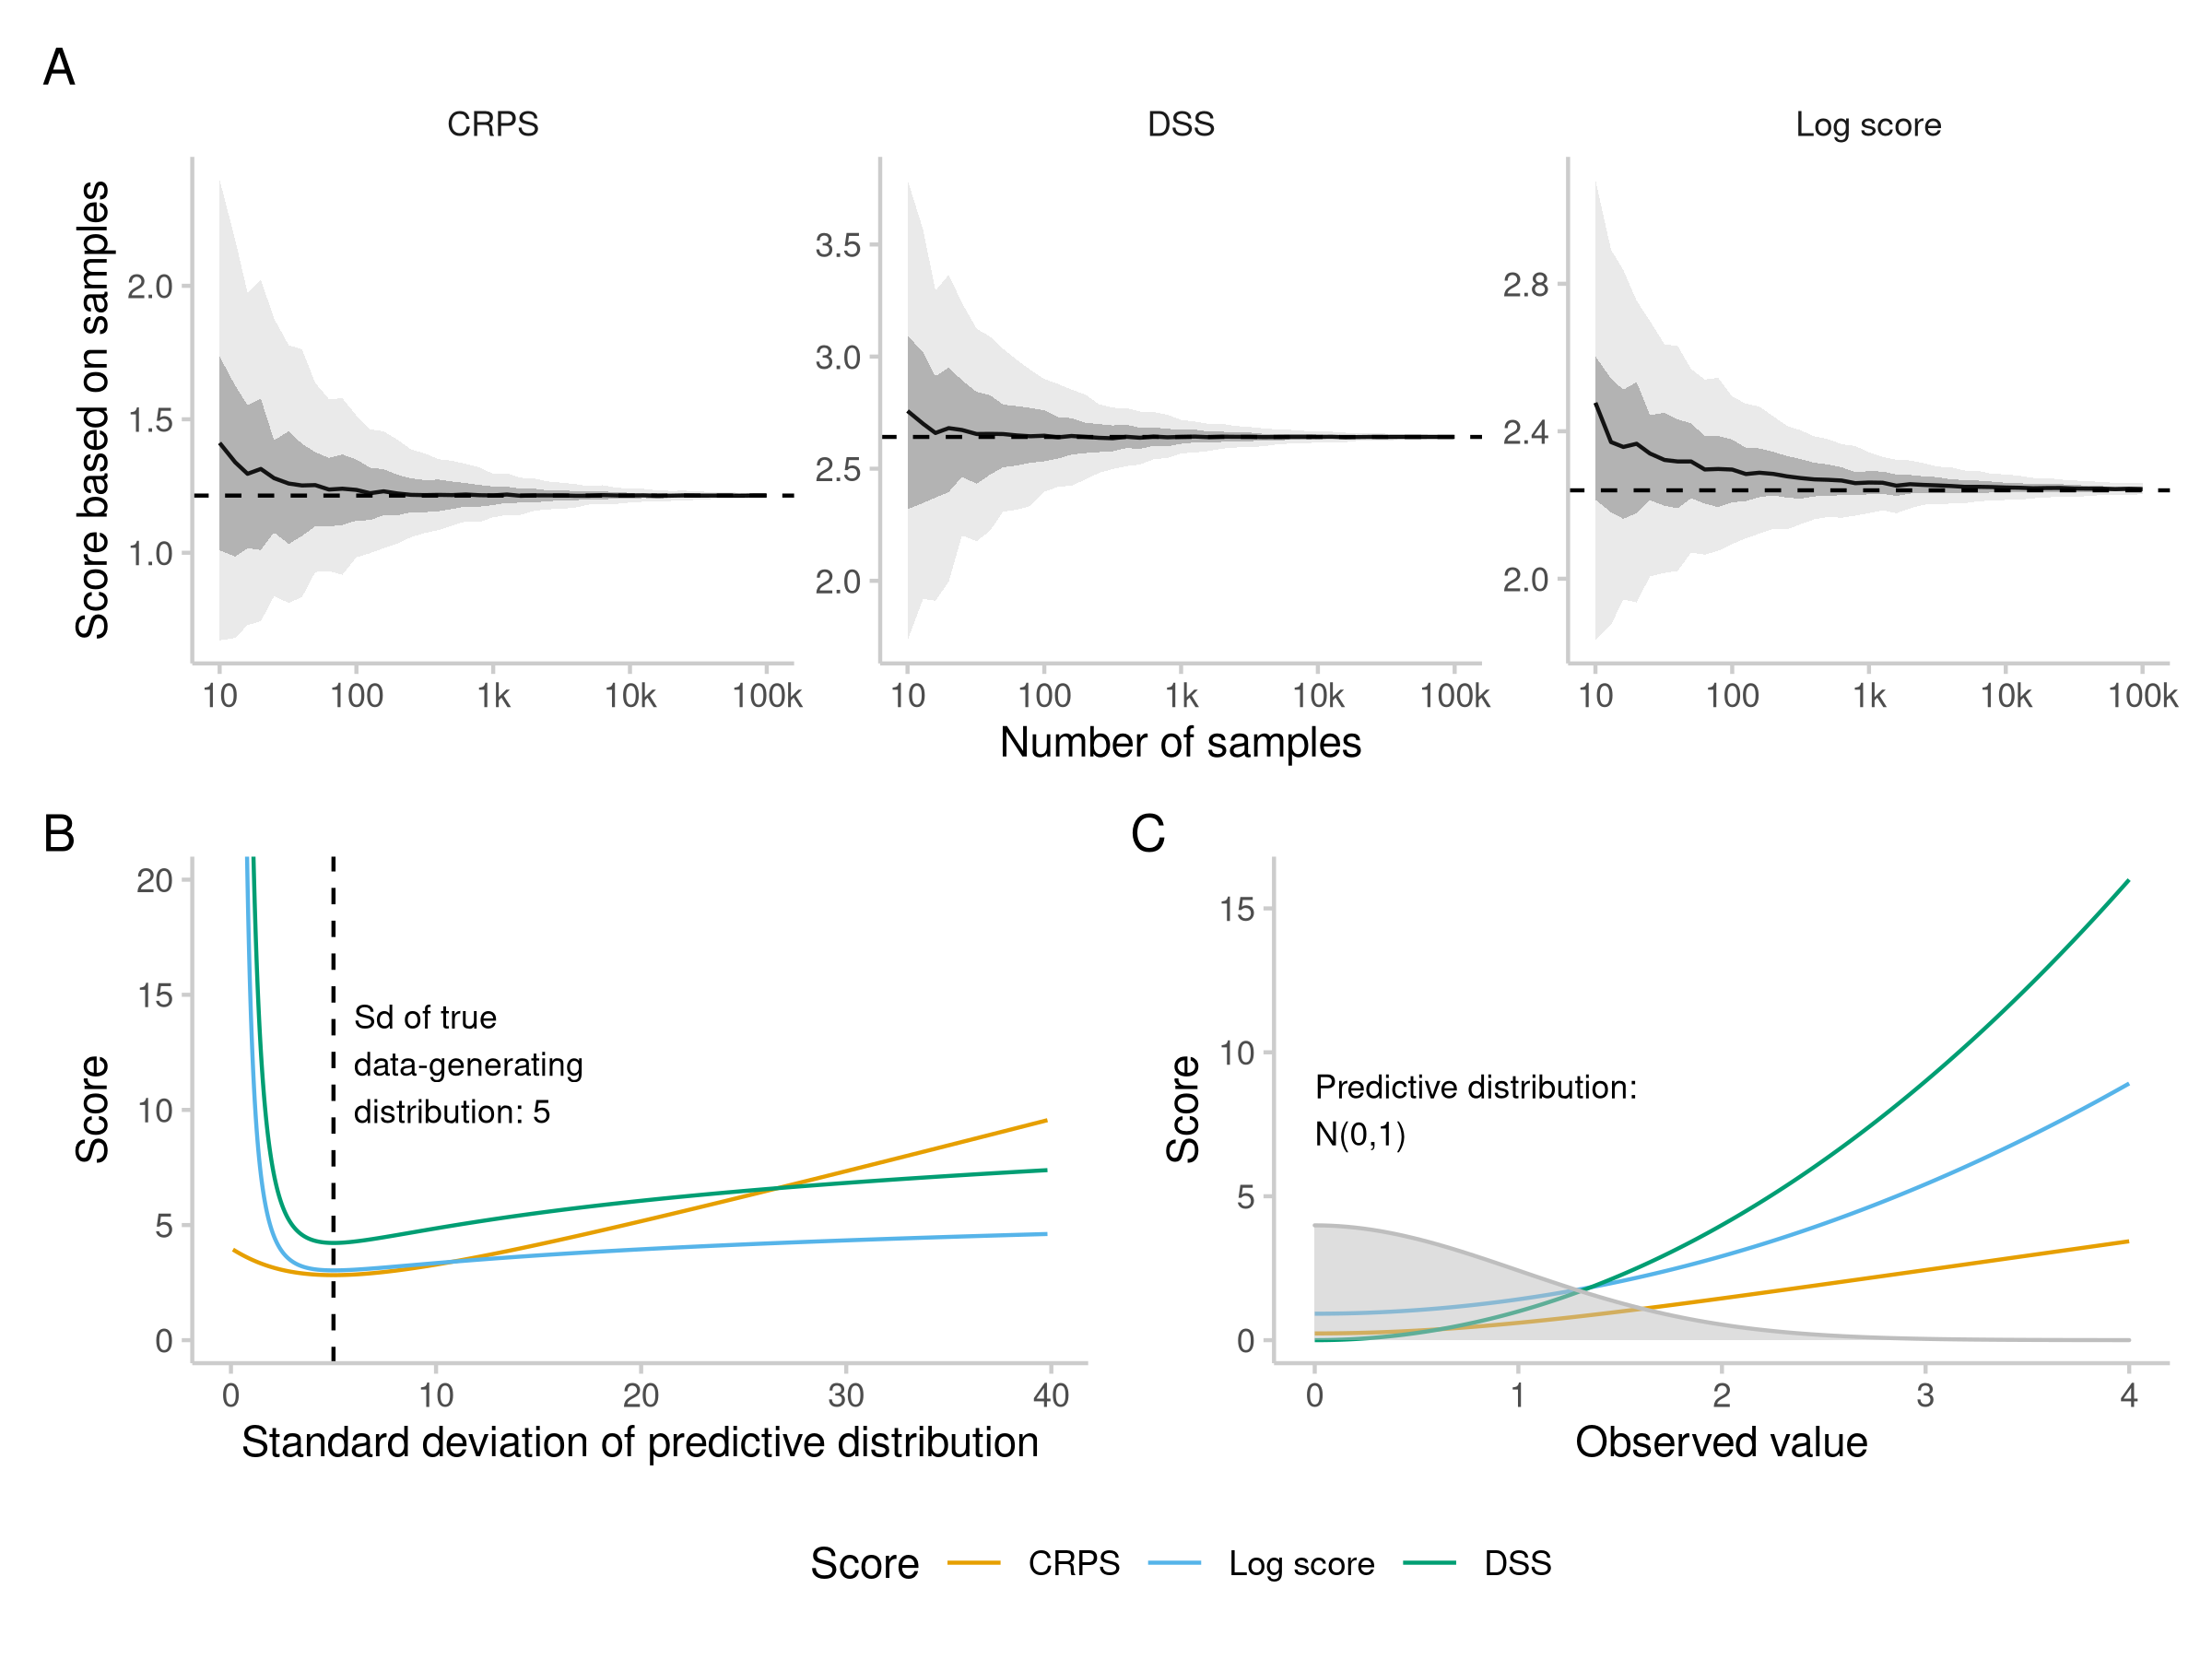
\includegraphics[width=1\linewidth]{output/score-convergence-outliers} 

}

\caption[Top]{Top: Estimation of scores from predictive samples (adapted from \citep{jordanEvaluatingProbabilisticForecasts2019}). Scores were computed based on samples of differing size (from 10 to 100,000). This was repeated 500 times for each sample size. The black line is the mean score across the 500 repetitions, shaded areas represent 50\% and 90\% intervals, and the dashed line represents the true calculated score.  Bottom left: Change in score when the uncertainty of the predictive distribution is changed. The true distribution is N(0,5) with the true standard deviation marked with a dashed line, while the standard deviation of the predictive distribution is varied along the x-axis. Log score and DSS clearly punish overconfidence much more severely than underconfidence. Bottom right: Score achieved for a standard normal predictive distribution (illustrated in grey) and different true observed values. Log score and DSS punish instances more harshly where the observed value is far away from the predictive distribution.}\label{fig:score-convergence}
\end{figure}
\end{CodeChunk}

\hypertarget{overconfidence-underconfidence-and-outliers}{%
\paragraph{Overconfidence, underconfidence and
outliers}\label{overconfidence-underconfidence-and-outliers}}

Proper scoring rules differ in how they penalise over- or underconfident
forecasts. The log score and the DSS penalise overconfidence much more
severely than underconfidence, while the CRPS does not distinguish
between over- and underconfidence and penalises both rather leniently
\citep{macheteContrastingProbabilisticScoring2012} (see Figure
\ref{fig:score-convergence}B, left panel). Similarly, the CRPS is
relatively lenient with regards to outlier predictions compared to the
log score and the DSS (see Figure \ref{fig:score-convergence}B, right
panel). The CRPS, which can be thought of as a generalisation of the
absolute error to a predictive distribution, scales linearly with the
distance between forecast distribution and true value. The log score, on
the other hand, as the negative logarithm of the predictive density
evaluated at the observed value, can quickly tend to infinity if the
probability assigned to the observed outcome is close to zero. Whether
or not harsh penalisation of overconfidence and bad predictions is
desirable or not depends of course on the setting. If, for example, one
wanted to forecast hospital bed capacity, it may be prudent to score
forecasts using a log score as one might prefer to be too cautious
rather than too confident.

\hypertarget{localglobal}{%
\paragraph{Sensitivity to distance - local vs. global
scores}\label{localglobal}}

The CRPS and the DSS are so-called global scoring rules, which means
that the score is sensitive to the distance of the entire predictive
distribution from the observed value. The log score, on the other hand,
is local and the resulting score depends only on the probability density
assigned to the actual outcome, ignoring the rest of the predictive
distribution (see Figure \ref{fig:score-locality}). Sensitivity to
distance (taking the entire predictive distribution into account) may be
a desirable property in most settings that involve decision making. A
prediction which assigns high probability to results far away from the
observed value is arguably less useful than a forecast which assigns a
lot of probability mass to values closer to the observed outcome (the
probability assigned to the actual outcome being equal for both
forecasts). The log score is only implicitly sensitive to distance in
expectation if we assume that values close to the observed value are
actually more likely to occur. The fact that the log score only depends
on the outcome that actually realised, however, may make it more
appropriate for inferential purposes (see
\citep{winklerScoringRulesEvaluation1996}) and it is commonly used in
Bayesian statistics
\citep{gelmanUnderstandingPredictiveInformation2014}.

\begin{CodeChunk}
\begin{figure}

{\centering 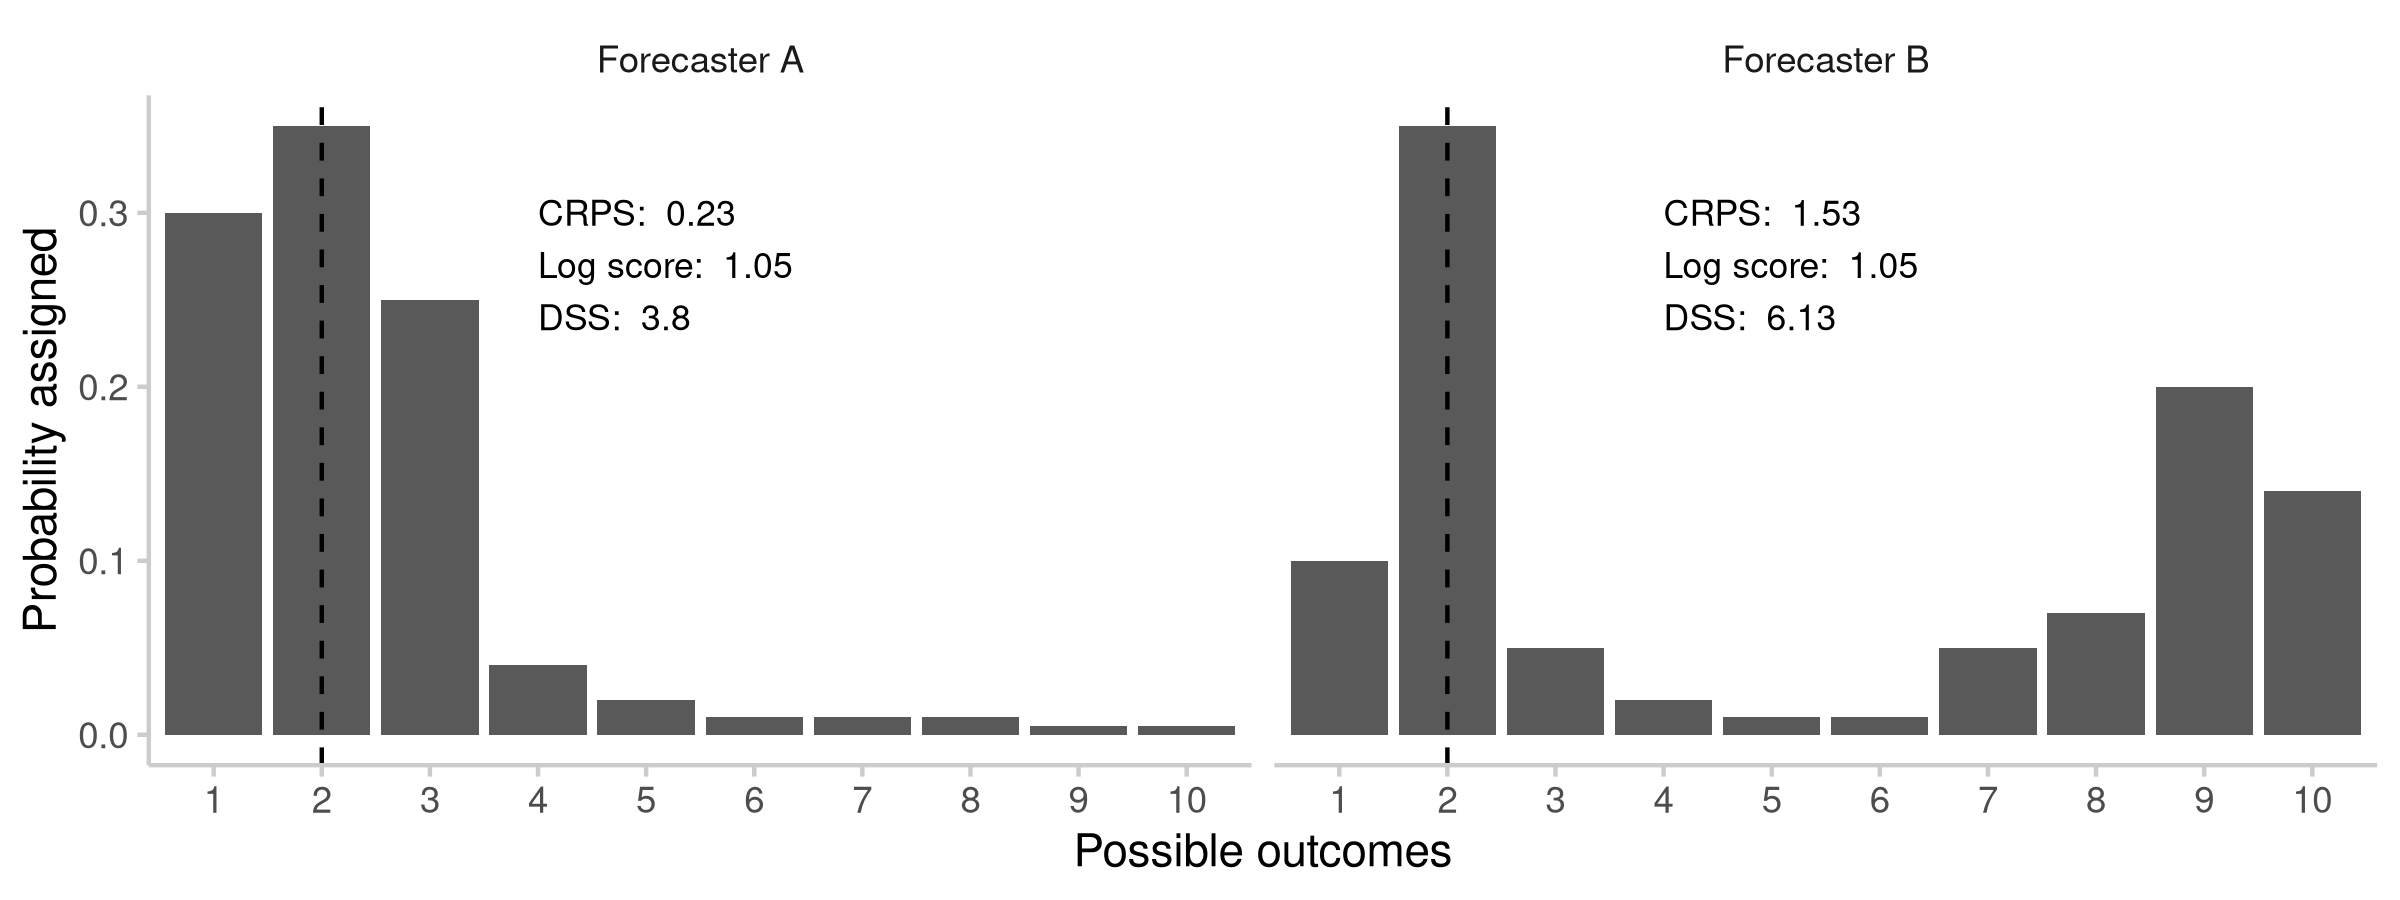
\includegraphics[width=1\linewidth]{output/score-locality} 

}

\caption[Probabilities assigned by two hypothetical forecasters, A and B, to the possible number of goals in a football match]{Probabilities assigned by two hypothetical forecasters, A and B, to the possible number of goals in a football match. The true number later observed, 2, is marked with a dashed line. Both forecasters assign a probability of 0.35 to the observed outcome, 2. Forecaster A's prediction is centred around the observed value, while Forecaster B assigns significant probability to outcomes far away from the observed value. Judged by a local score like the Log Score, both forecasters receive the same score. A global score like the CRPS and the DSS penalises forecaster B more severely.}\label{fig:score-locality}
\end{figure}
\end{CodeChunk}

\hypertarget{sensitivity-to-the-order-of-magnitude-of-the-forecast-quantity}{%
\paragraph{Sensitivity to the order of magnitude of the forecast
quantity}\label{sensitivity-to-the-order-of-magnitude-of-the-forecast-quantity}}

Average scores usually scale with the order of magnitude of the quantity
we try to forecast (as the variance of the data-generating distribution
usually increases with the mean). Figure \ref{fig:score-scale}
illustrates the effect of an increase in scale of the forecast target on
average scores. This relation makes it harder to compare forecasts for
very different targets, or assess average performance if the quantity of
interest varies substantially over time. Average scores tend to be
dominated by forecasts for targets with high absolute numbers. This is
especially the case for the CRPS (as a generalisation of the absolute
error), for which average scores tend to increase strongly with the
order of magnitude of the quantity to forecast (see Figure
\ref{fig:score-scale}. The log score and the DSS tend to be more robust
against this effect and on average increase more slowly with an increase
in the variance of the forecast target.

\begin{CodeChunk}
\begin{figure}

{\centering 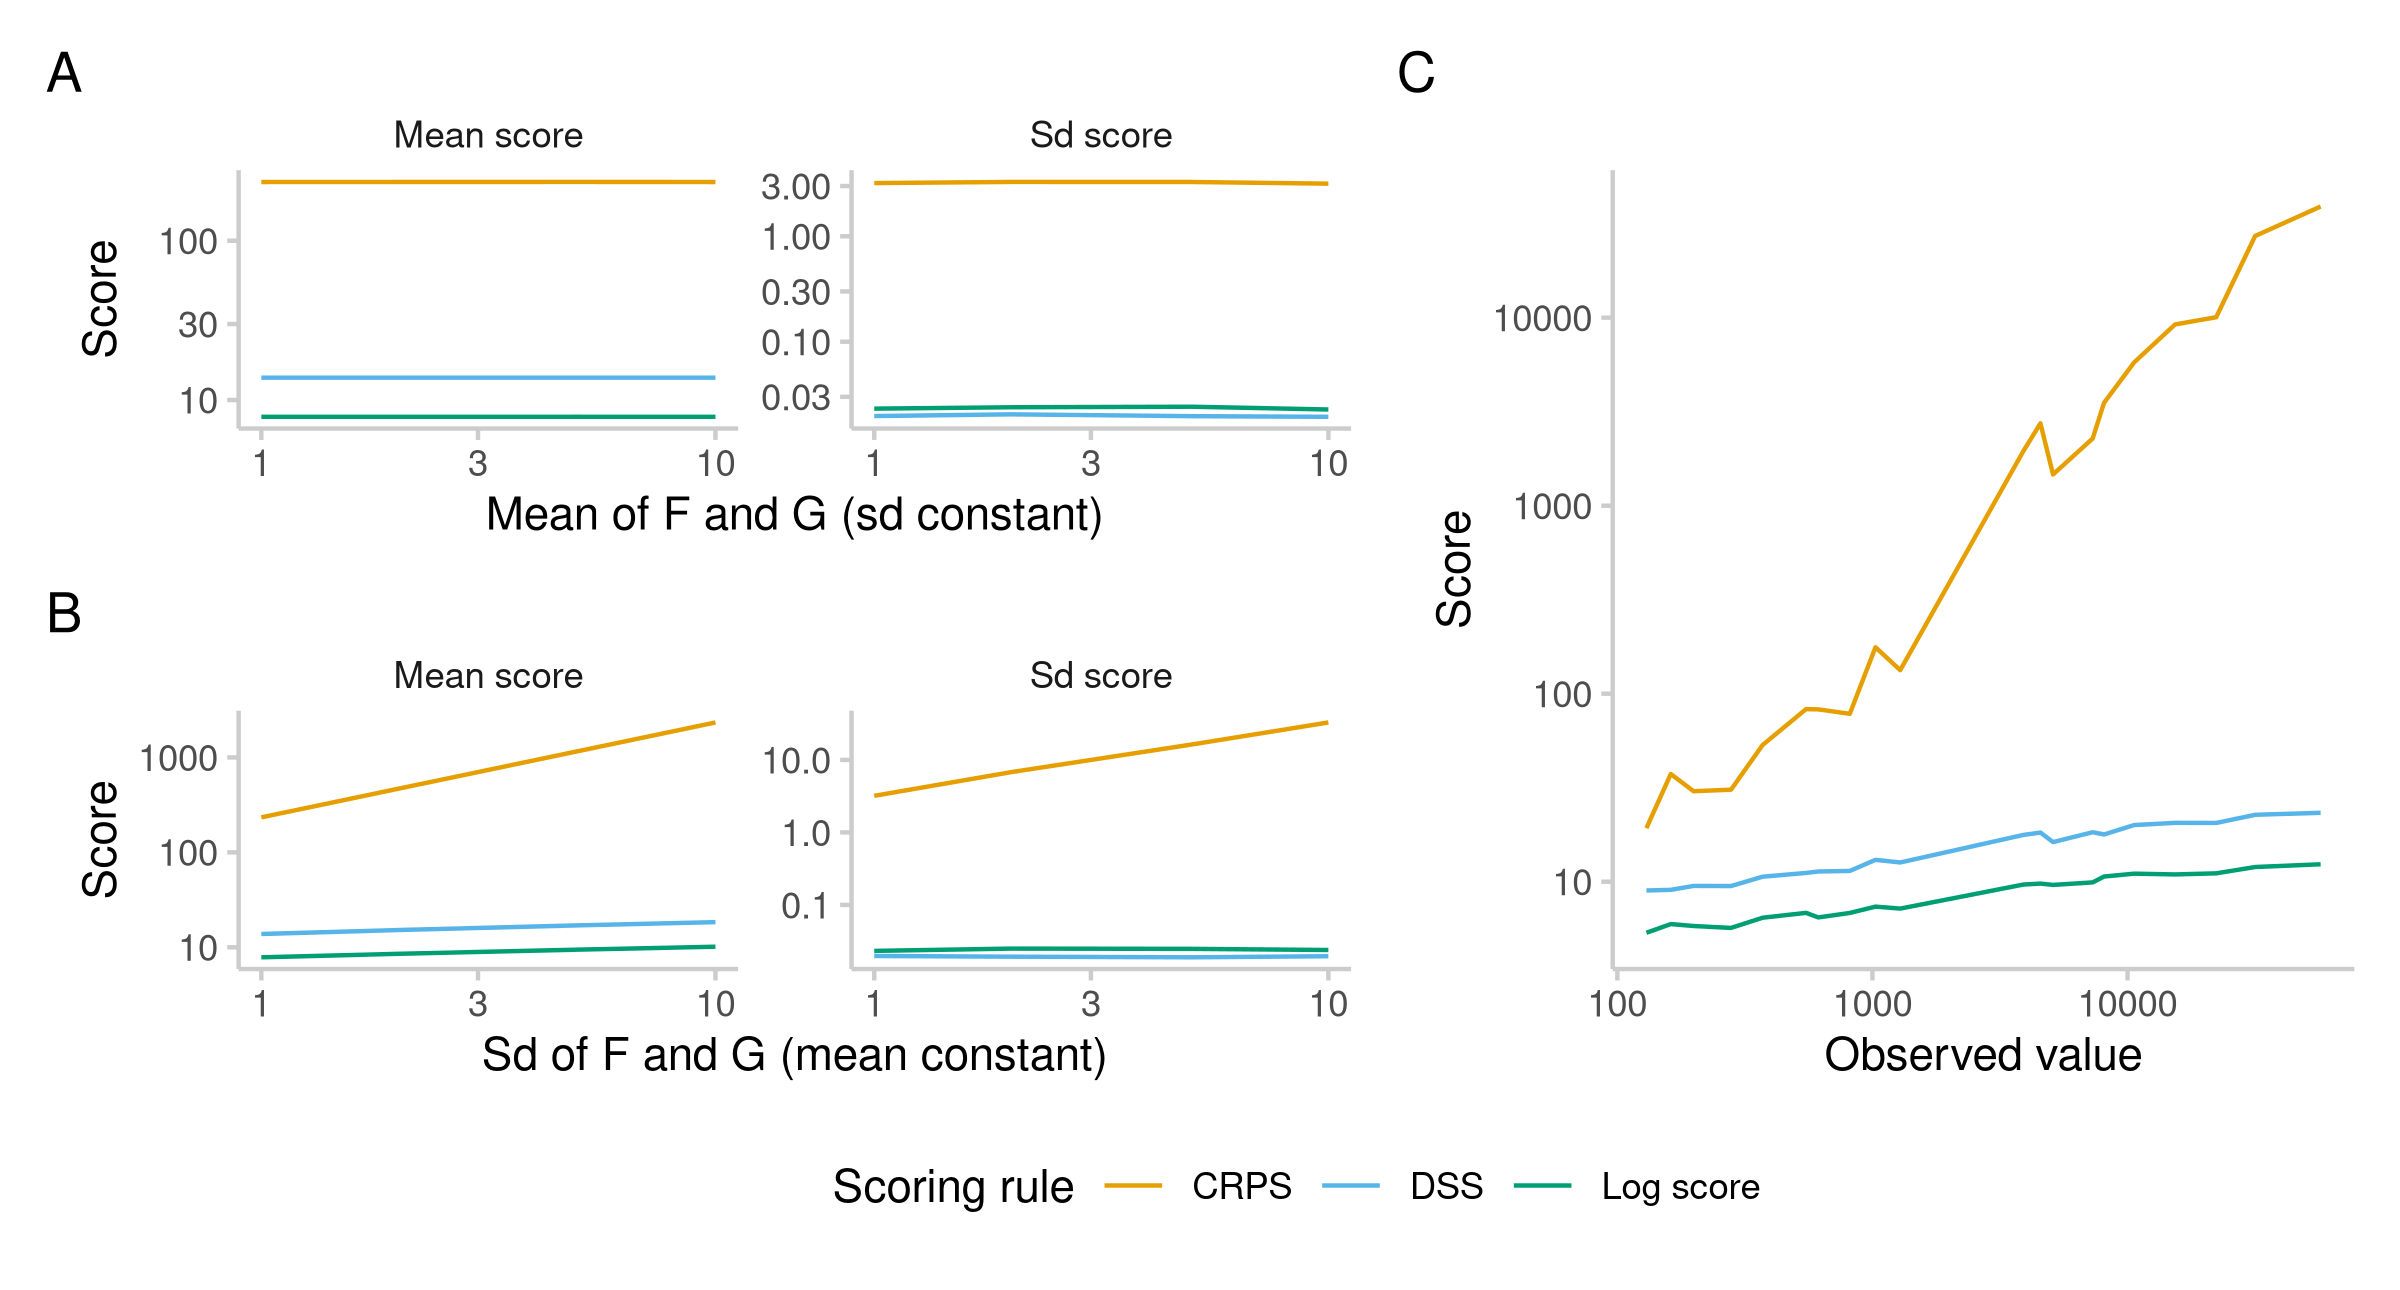
\includegraphics[width=1\linewidth]{output/illustration-effect-scale} 

}

\caption[Scores depend on the variability of the data and therefore implicitly on the order of magnitude of the observed value]{Scores depend on the variability of the data and therefore implicitly on the order of magnitude of the observed value. A: Mean and standard deviation of scores from a simulation of perfect forecasts with predictive distribution $F$ equal to the true data-generating distribution $G$. The standard deviation of the two distributions was held constant at $\sigma$, and for different mean values $\mu$ 100 pairs of forecasts and observations were simulated. Every simulated forecast consisted of 1000 draws from the data-generating distribution $G$ and 5000 draws from the (same) predictive distribution $F$. For all three scoring rules, mean and sd of the calculated scores stay constant regardless of the mean $\mu$ of $F$ and $G$. B: Same setup, but now the mean of $F$ and $G$ was held constant at $\mu = 1$ and the standard deviation $\sigma$ was varied. Average scores increase for all three scoring rules, but most strongly for the CRPS. Standard deviations of the estimated scores stay roughly constant for the DSS and log score, but also increase for the CRPS. C: Scores for forecasts of COVID-19 cases and deaths from the European Forecast Hub ensemble based on the example data provided in the package.}\label{fig:score-scale}
\end{figure}
\end{CodeChunk}

\hypertarget{wis}{%
\subsubsection{Proper scoring rule for quantile-based forecasts
(WIS)}\label{wis}}

For forecasts in an interval or quantile format, \pkg{scoringutils}
offers the weighted interval score (WIS)
\citep{bracherEvaluatingEpidemicForecasts2021}. The WIS has very similar
properties to the CRPS and can be thought of as a quantile-based
approximation. For an increasing number of equally-spaced prediction
intervals the WIS converges to the CRPS. One additional benefit of the
WIS is that it can easily be decomposed into three additive components:
an uncertainty penalty (called dispersion or sharpness penalty) for the
width of a prediction interval and penalties for over- and
underprediction (if a value falls outside of a prediction interval).

\hypertarget{proper-scoring-rules-for-binary-outcomes-bs-and-log-score}{%
\subsubsection{Proper scoring rules for binary outcomes (BS and log
score)}\label{proper-scoring-rules-for-binary-outcomes-bs-and-log-score}}

Binary forecasts can be scored using the Brier score (BS) or the log
score. The Brier score \citep{brierVERIFICATIONFORECASTSEXPRESSED1950}
corresponds to the squared difference between the given probability and
the outcome (either 0 or 1) and equals the ranked probability score for
the case of only two possible outcomes
\citep{epsteinScoringSystemProbability1969, murphyNoteRankedProbability1971a}.
The log score corresponds to the log of the probability assigned to the
observed outcome. Just as with continuous forecasts, the log score
penalises overconfidence much more harshly than underconfidence. The
Brier score, on the other hand, penalises over- and underconfidence
similarly \citep{macheteContrastingProbabilisticScoring2012} and is more
forgiving of outlier predictions.

\hypertarget{pairwisetheory}{%
\subsection{Pairwise comparisons}\label{pairwisetheory}}

Raw scores for different forecasting models are not directly comparable
in the case of missing forecasts, as forecasting targets usually differ
in their characteristics (e.g.~the scale of the forecast target, how
difficult targets are to forecast etc.). One way to mitigate this are
relative skill scores based on pairwise comparisons
\citep{cramerEvaluationIndividualEnsemble2021}. Models enter a `pairwise
tournament', where all possible pairs of models are compared based on
the overlapping set of available forecasts common to both models
(omitting comparisons where there is no overlapping set of forecasts).
For every pair, the ratio of the mean scores of both models is computed.
The relative skill score of a model is then the geometric mean of all
mean score ratios which involve that model. This gives us an indicator
of performance relative to all other models, with the orientation
depending on the score used (e.g.~for the proper scoring rules presented
above, a relative skill score below 1 indicates better performance). As
two models can only be fairly compared if they have overlapping
forecasts it is advisable to only compare forecasts that are at least
50\% complete (to avoid comparisons of models that have no overlapping
forecasts). Furthermore, pairwise comparisons are only possible if all
scores have the same sign. One can also compute a scaled relative skill
score by providing a baseline model. All individual relative skill
scores are then scaled by (i.e.~divided by) the relative score of the
baseline model.

It is in principle possible to compute p-values to determine whether two
models perform significantly differently. \pkg{scoringutils} allows to
compute these using either the Wilcoxon rank sum test (also known as
Mann-Whitney-U test) \citep{mannTestWhetherOne1947} or a permutation
test. In practice, this is complicated by the fact that both tests
assume independent observations. In reality, however, forecasts by a
model may be correlated across time or another dimension (e.g.~if a
forecaster has a bad day, they might perform badly across different
targets for a given forecast date). P-values may therefore be too
liberal in suggesting significant differences where there aren't any.
One way to mitigate this is to aggregate observations over a category
where one suspects correlation (for example averaging across all
forecasts made on a given date) before making pairwise comparisons. A
test that is performed on aggregate scores will likely be more
conservative.

\hypertarget{evaluation-example}{%
\section{Evaluating forecasts using
scoringutils}\label{evaluation-example}}

This section details the core features of \pkg{scoringutils}, explains
the expected data input formats and illustrates how to evaluate and
compare forecasts using the example data provided in the package.
\pkg{scoringutils} offers comprehensive functionality to conduct a
forecast evaluation and allows users to check inputs, score forecasts
and visualise results. Most functions operate on a
\texttt{data.frame}-based format, but the package also provides a set of
function to score individual forecasts directly which operate on
vectors/matrices. These will not be discussed in this paper and we refer
to the vignettes and package documentation for further
information\footnote{https://epiforecasts.io/scoringutils/}. Some helper
functions for data-handling, as well as example data sets and tables
with additional information about available scoring metrics are also
included in the package.

\hypertarget{example-data}{%
\subsection{Example data}\label{example-data}}

The example data included in the package and used in this paper consists
of one to three week ahead forecasts made between May and September 2021
for COVID-19 cases and deaths from four different forecasting models. It
represents a small subset of short-term predictions for COVID-19 cases
and deaths submitted to the European Forecast Hub
\citep{europeancovid-19forecasthubEuropeanCovid19Forecast2021}. The
European Forecast Hub each week collates, aggregates and evaluates one
to four week ahead predictions of different COVID-19 related targets
submitted by different research groups. Forecasts are submitted in a
quantile-based format with a set of 22 quantiles plus the median
(\(0.01, 0.025, 0.05, ..., 0.5, ... 0.95, 0.975, 0.99\)). The full
official hub evaluations, which also use \pkg{scoringutils}, can be seen
at \url{https://covid19forecasthub.eu/}.

In the following, we will use the \code{glimpse()} function from the
package \pkg{tibble} to display outputs more concisely. After loading
the \pkg{scoringutils} package we can directly inspect the example data:

\begin{CodeChunk}
\begin{CodeInput}
R> library(scoringutils)
R> library(tibble) 
R> 
R> example_quantile |>
+   na.omit() |>
+   glimpse()
\end{CodeInput}
\begin{CodeOutput}
Rows: 20,401
Columns: 10
$ location        <chr> "DE", "DE", "DE", "DE", "DE", "DE", "DE", "D~
$ target_end_date <date> 2021-05-08, 2021-05-08, 2021-05-08, 2021-05~
$ target_type     <chr> "Cases", "Cases", "Cases", "Cases", "Cases",~
$ true_value      <dbl> 106987, 106987, 106987, 106987, 106987, 1069~
$ location_name   <chr> "Germany", "Germany", "Germany", "Germany", ~
$ forecast_date   <date> 2021-05-03, 2021-05-03, 2021-05-03, 2021-05~
$ quantile        <dbl> 0.010, 0.025, 0.050, 0.100, 0.150, 0.200, 0.~
$ prediction      <int> 82466, 86669, 90285, 95341, 99171, 102990, 1~
$ model           <chr> "EuroCOVIDhub-ensemble", "EuroCOVIDhub-ensem~
$ horizon         <dbl> 1, 1, 1, 1, 1, 1, 1, 1, 1, 1, 1, 1, 1, 1, 1,~
\end{CodeOutput}
\end{CodeChunk}

\hypertarget{expected-input-formats-and-data-checking}{%
\subsection{Expected input formats and data
checking}\label{expected-input-formats-and-data-checking}}

Depending on the format of the forecast, a \texttt{data.frame} (or
similar) is required for most functions with column names as shown in
Table \ref{tab:column-requirements}. Point forecasts are defined as
forecasts that follow a quantile-based format (and can be mixed with
quantile-based forecasts), but which have an \texttt{NA} value in the
column \texttt{"quantile"}.

\begin{CodeChunk}
\begin{table}

\caption{\label{tab:column-requirements}Overview of the columns required for different input formats.}
\centering
\begin{tabular}[t]{l>{\raggedright\arraybackslash}p{6cm}>{\raggedright\arraybackslash}p{3.7cm}}
\toprule
Format & Required columns & Example data\\
\midrule
\cellcolor{gray!6}{quantile-based} & \cellcolor{gray!6}{'true\_value', 'prediction', 'quantile'} & \cellcolor{gray!6}{example\_quantile}\\
\addlinespace
sample-based & 'true\_value', 'prediction', 'sample' & example\_integer, 
  example\_continuous\\
\addlinespace
\cellcolor{gray!6}{binary} & \cellcolor{gray!6}{'true\_value', 'prediction'} & \cellcolor{gray!6}{example\_binary}\\
\addlinespace
point-forecasts & like quantile-based, but with 
 NA in the 'quantile' column & example\_point\\
\addlinespace
\cellcolor{gray!6}{pairwise-comparisons} & \cellcolor{gray!6}{additionally a column 'model'} & \cellcolor{gray!6}{\textasciitilde{}}\\
\bottomrule
\end{tabular}
\end{table}

\end{CodeChunk}

Additional columns may be present to indicate a grouping of forecasts. A
combination of different columns should uniquely define the unit of a
single forecast, meaning that a single forecast is defined by the
combination of values in the other columns. For example, a single
forecast could be uniquely defined by a model name, a location, a
forecast date and a forecast horizon.

The function \code{check\_forecasts()} allows to check whether input
data conforms to the function requirements and returns a list with
entries that provide information on what \pkg{scoringutils} infers from
the data.

\begin{CodeChunk}
\begin{CodeInput}
R> check_forecasts(example_quantile)
\end{CodeInput}
\begin{CodeOutput}
Your forecasts seem to be for a target of the following type:
$target_type
[1] "integer"

and in the following format:
$prediction_type
[1] "quantile"

The unit of a single forecast is defined by:
$forecast_unit
[1] "location"        "target_end_date" "target_type"    
[4] "location_name"   "forecast_date"   "model"          
[7] "horizon"        

Cleaned data, rows with NA values in prediction or true_value removed:
$cleaned_data
       location target_end_date target_type true_value location_name
    1:       DE      2021-05-08       Cases     106987       Germany
    2:       DE      2021-05-08       Cases     106987       Germany
    3:       DE      2021-05-08       Cases     106987       Germany
    4:       DE      2021-05-08       Cases     106987       Germany
    5:       DE      2021-05-08       Cases     106987       Germany
   ---                                                              
20397:       IT      2021-07-24      Deaths         78         Italy
20398:       IT      2021-07-24      Deaths         78         Italy
20399:       IT      2021-07-24      Deaths         78         Italy
20400:       IT      2021-07-24      Deaths         78         Italy
20401:       IT      2021-07-24      Deaths         78         Italy
       forecast_date quantile prediction                 model
    1:    2021-05-03    0.010      82466 EuroCOVIDhub-ensemble
    2:    2021-05-03    0.025      86669 EuroCOVIDhub-ensemble
    3:    2021-05-03    0.050      90285 EuroCOVIDhub-ensemble
    4:    2021-05-03    0.100      95341 EuroCOVIDhub-ensemble
    5:    2021-05-03    0.150      99171 EuroCOVIDhub-ensemble
   ---                                                        
20397:    2021-07-12    0.850        352  epiforecasts-EpiNow2
20398:    2021-07-12    0.900        397  epiforecasts-EpiNow2
20399:    2021-07-12    0.950        499  epiforecasts-EpiNow2
20400:    2021-07-12    0.975        611  epiforecasts-EpiNow2
20401:    2021-07-12    0.990        719  epiforecasts-EpiNow2
       horizon
    1:       1
    2:       1
    3:       1
    4:       1
    5:       1
   ---        
20397:       2
20398:       2
20399:       2
20400:       2
20401:       2

Number of unique values per column per model:
$unique_values
                   model location target_end_date target_type
1: EuroCOVIDhub-ensemble        4              12           2
2: EuroCOVIDhub-baseline        4              12           2
3:  epiforecasts-EpiNow2        4              12           2
4:       UMass-MechBayes        4              12           1
   true_value location_name forecast_date quantile prediction horizon
1:         96             4            11       23       3969       3
2:         96             4            11       23       3733       3
3:         95             4            11       23       3903       3
4:         48             4            11       23       1058       3

$messages
[1] "144 values for `prediction` are NA in the data provided and the corresponding rows were removed. This may indicate a problem if unexpected."
\end{CodeOutput}
\end{CodeChunk}

The values stored in the list elements \code{target_type} and
\code{prediction_type} refer to type of the forecast and the target
variable. \code{forecast_unit} contains a vector of the columns which
\pkg{scoringutils} thinks denote the unit of a single forecast. This
means that in this instance a single forecast (with a set of 23
quantiles) can uniquely be identified by the values in the columns
``location'', ``target\_end\_date'', ``target\_type'',
``location\_name'', ``forecast\_date'', ``model'', ``horizon''. In this
example, having ``location'' as well as ``location\_name'' included does
not make a difference, as they contain duplicated information. In
general, however, it is strongly advised to remove all unnecessary
columns that do not help identify a single forecast.
\code{unique_values} gives an overview of the number of unique values
per column across the entire data set, providing a first hint as to
whether the forecast set is complete. \code{messages} or \code{warnings}
show messages and warnings created when checking the data.

\hypertarget{visualising-forecast-data}{%
\subsection{Visualising forecast data}\label{visualising-forecast-data}}

It is helpful to start the evaluation process by examining forecast
availability, as missing forecasts can impact the evaluation if
missingness correlates with performance. The function
\code{avail_forecasts()} returns information about the number of
available forecasts, given a level of summary that can be specified
through the \code{by} argument. For example, to see how many forecasts
there are per model and target\_type, we can run

\begin{CodeChunk}
\begin{CodeInput}
R> avail_forecasts(data = example_integer, 
+                 by = c("model", "target_type"))
\end{CodeInput}
\begin{CodeOutput}
                   model target_type Number forecasts
1: EuroCOVIDhub-ensemble       Cases              128
2: EuroCOVIDhub-baseline       Cases              128
3:  epiforecasts-EpiNow2       Cases              128
4: EuroCOVIDhub-ensemble      Deaths              128
5: EuroCOVIDhub-baseline      Deaths              128
6:       UMass-MechBayes      Deaths              128
7:  epiforecasts-EpiNow2      Deaths              119
\end{CodeOutput}
\end{CodeChunk}

and visualise results using the function
\code{plot\_avail\_forecasts()}. The plot resulting from running the
following code is displayed in Figure \ref{fig:avail-forecasts-plot}.

\begin{CodeChunk}
\begin{CodeInput}
R> library(ggplot2)
R> 
R> avail_forecasts(data = example_integer, 
+                 by = c("model", "target_type", "forecast_date")) |>
+   plot_avail_forecasts(x = "forecast_date", 
+                        show_numbers = FALSE) + 
+   facet_wrap(~ target_type) + 
+   labs(y = "Model", x = "Forecast date") 
\end{CodeInput}
\begin{figure}[!h]

{\centering 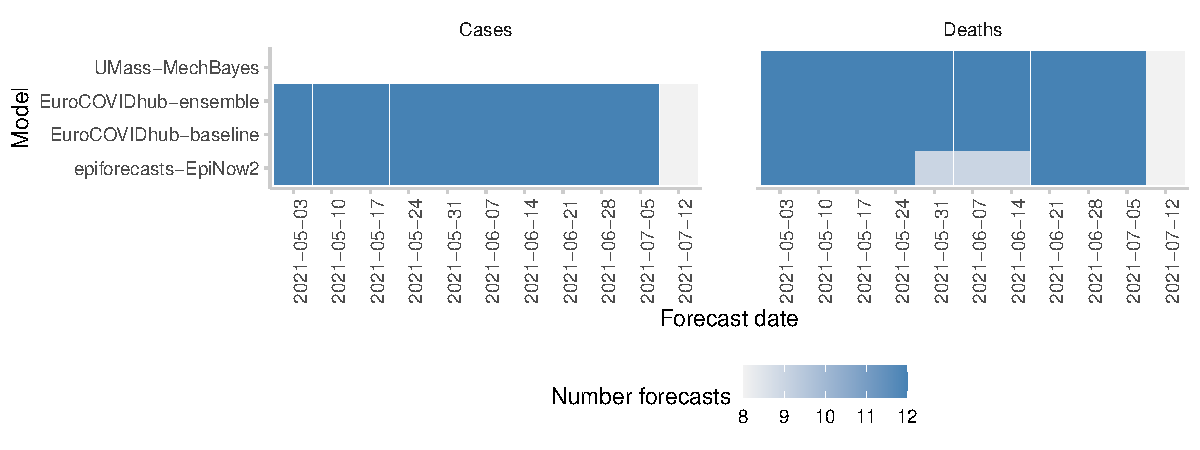
\includegraphics[width=1\linewidth]{manuscript_files/figure-latex/avail-forecasts-plot-1} 

}

\caption[Overview of the number of available forecasts]{Overview of the number of available forecasts.}\label{fig:avail-forecasts-plot}
\end{figure}
\end{CodeChunk}

The forecasts and observed values themselves can be visualised using the
\code{plot\_predictions()} function and its \code{make\_na()} helper
function. \code{make\_na()} represents a form of filtering, but instead
of filtering entire rows, the relevant entries in the columns
``prediction'' or ``true\_value'' are made \texttt{NA}. This allows the
user to filter observations and forecasts independently. In order to be
able to facet the plot correctly, \code{plot\_predictions()} has a an
additional \texttt{by} argument in which the user needs to specify all
columns relevant for facetting. In order to be To display, for example,
short-term forecasts for COVID-19 cases and deaths made by the
EuroCOVIDhub-ensemble model on June 28 2021 as well as 5 weeks of prior
data, we can call the following. The resulting plot is shown in Figure
\ref{fig:forecast-visualisation}.

\begin{CodeChunk}
\begin{CodeInput}
R> example_quantile %>%
+   make_na(what = "truth", 
+           target_end_date > "2021-07-15",
+           target_end_date <= "2021-05-22") %>%
+   make_na(what = "forecast", 
+           model != "EuroCOVIDhub-ensemble",
+           forecast_date != "2021-06-28") %>%
+   plot_predictions(x = "target_end_date", by = c("target_type", "location")) +
+   aes(colour = model, fill = model) +
+   facet_wrap(target_type ~ location, ncol = 4, scales = "free_y") +
+   labs(x = "Target end date")
\end{CodeInput}
\begin{figure}[!h]

{\centering 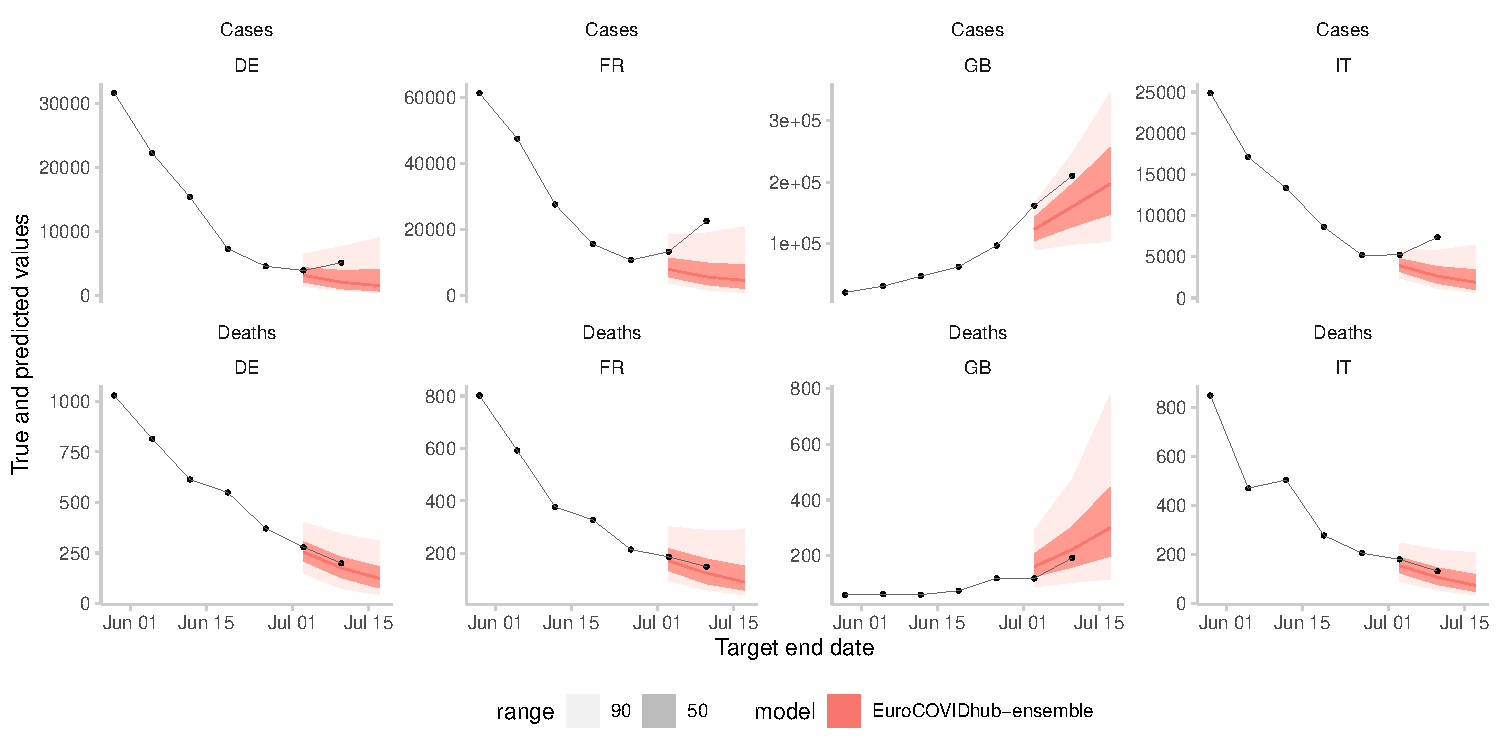
\includegraphics[width=1\linewidth]{manuscript_files/figure-latex/forecast-visualisation-1} 

}

\caption[Short-term forecasts for COVID-19 cases and deaths made by the EuroCOVIDhub-ensemble model on June 28 2021]{Short-term forecasts for COVID-19 cases and deaths made by the EuroCOVIDhub-ensemble model on June 28 2021.}\label{fig:forecast-visualisation}
\end{figure}
\end{CodeChunk}

\subsection[Scoring forecasts with score()]{Scoring forecasts with
\code{score()}}\label{scoring}

The function \code{score()} evaluates predictions against observed
values and automatically applies the appropriate scoring metrics
depending on the input data.

We can simply call:

\begin{CodeChunk}
\begin{CodeInput}
R> score(example_quantile) |>
+   glimpse()
\end{CodeInput}
\begin{CodeOutput}
Rows: 20,401
Columns: 18
$ location           <chr> "DE", "DE", "DE", "DE", "DE", "DE", "DE",~
$ target_end_date    <date> 2021-05-08, 2021-05-08, 2021-05-08, 2021~
$ target_type        <chr> "Cases", "Cases", "Cases", "Cases", "Case~
$ location_name      <chr> "Germany", "Germany", "Germany", "Germany~
$ forecast_date      <date> 2021-05-03, 2021-05-03, 2021-05-03, 2021~
$ model              <chr> "EuroCOVIDhub-baseline", "EuroCOVIDhub-ba~
$ horizon            <dbl> 1, 1, 1, 1, 1, 1, 1, 1, 1, 1, 1, 1, 1, 1,~
$ range              <dbl> 0, 10, 10, 20, 20, 30, 30, 40, 40, 50, 50~
$ interval_score     <dbl> 25620.00, 25599.50, 25599.50, 25481.00, 2~
$ dispersion         <dbl> 0.00, 184.50, 184.50, 556.00, 556.00, 816~
$ underprediction    <dbl> 0, 0, 0, 0, 0, 0, 0, 0, 0, 0, 0, 0, 0, 0,~
$ overprediction     <dbl> 25620, 25415, 25415, 24925, 24925, 24454,~
$ coverage           <dbl> 0, 0, 0, 0, 0, 0, 0, 0, 0, 0, 0, 0, 0, 0,~
$ coverage_deviation <dbl> 0.00, -0.10, -0.10, -0.20, -0.20, -0.30, ~
$ bias               <dbl> 0.95, 0.95, 0.95, 0.95, 0.95, 0.95, 0.95,~
$ quantile           <dbl> 0.500, 0.450, 0.550, 0.400, 0.600, 0.350,~
$ ae_median          <dbl> 25620, 25620, 25620, 25620, 25620, 25620,~
$ quantile_coverage  <lgl> TRUE, TRUE, TRUE, TRUE, TRUE, TRUE, TRUE,~
\end{CodeOutput}
\end{CodeChunk}

The above produces one score for every forecast. However, we usually
like to summarise scores to learn about average performance across
certain categories. This can be done using the function
\code{summarise\_scores()}, which returns one summarised score per
category (column name) specified in the argument \code{by}. To return,
for example, one score per model and forecast target, we can run the
following:

\begin{CodeChunk}
\begin{CodeInput}
R> score(example_quantile) |>
+   summarise_scores(by = c("model", "target_type")) |>
+   glimpse()
\end{CodeInput}
\begin{CodeOutput}
Rows: 7
Columns: 9
$ model              <chr> "EuroCOVIDhub-baseline", "EuroCOVIDhub-en~
$ target_type        <chr> "Cases", "Cases", "Cases", "Deaths", "Dea~
$ interval_score     <dbl> 28483.57465, 17943.82383, 20831.55662, 15~
$ dispersion         <dbl> 4102.50094, 3663.52458, 5664.37795, 91.40~
$ underprediction    <dbl> 10284.972826, 4237.177310, 3260.355639, 2~
$ overprediction     <dbl> 14096.100883, 10043.121943, 11906.823030,~
$ coverage_deviation <dbl> -0.11211957, -0.09785326, -0.06660326, 0.~
$ bias               <dbl> 0.09796875, -0.05640625, -0.07890625, 0.3~
$ ae_median          <dbl> 38473.60156, 24101.07031, 27923.81250, 23~
\end{CodeOutput}
\end{CodeChunk}

Summarised scores can then be visualised using the function
\code{scores\_table()}. In order to display scores it is often useful to
round the output to e.g.~two significant digits, which can be achieved
through another call of \code{summarise\_scores()}. The output of the
following is shown in Figure \ref{fig:score-table}:

\begin{CodeChunk}
\begin{CodeInput}
R> score(example_quantile) |>
+   summarise_scores(by = c("model", "target_type")) |>
+   summarise_scores(fun = signif, digits = 2) |>
+   plot_score_table(y = "model", by = "target_type") + 
+   facet_wrap(~ target_type)
\end{CodeInput}
\begin{figure}

{\centering 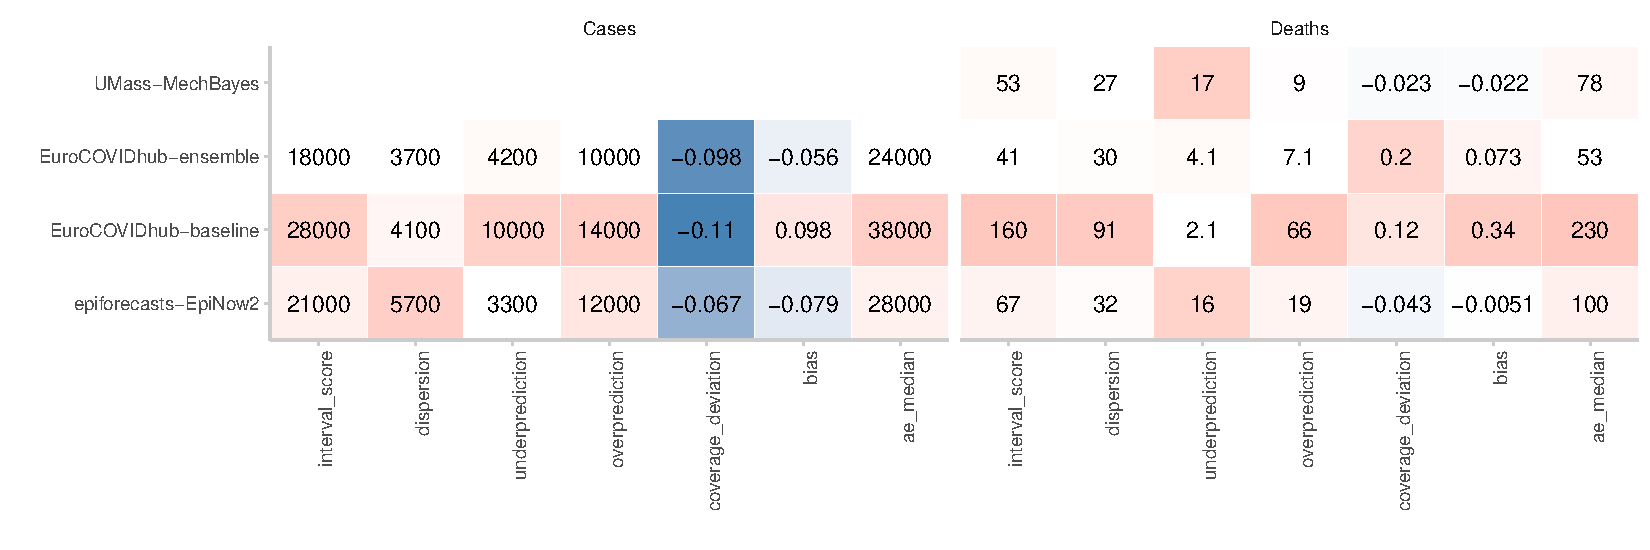
\includegraphics[width=1\linewidth]{manuscript_files/figure-latex/score-table-1} 

}

\caption[Coloured table to visualise the computed scores]{Coloured table to visualise the computed scores. Red colours indicate that a value is higher than ideal, blue indicates it is lower than ideal and the opacity indicates the strength of the deviation from the ideal.}\label{fig:score-table}
\end{figure}
\end{CodeChunk}

While \code{summarise\_scores()} accepts arbitrary summary functions,
care has to be taken when using something else than \code{mean()},
because scores may lose propriety when using other summary functions.
For example, the median of several individual scores (individually based
on a proper scoring rule) is usually not proper. A forecaster judged by
the median of several scores may be incentivised to misrepresent their
true belief in a way that is not true for the mean score.

The user must exercise additional caution and should usually avoid
aggregating scores across categories which differ much in the magnitude
of the quantity to forecast, as forecast errors usually increase with
the order of magnitude of the forecast target. In the given example,
looking at one score per model (i.e.~specifying
\code{summarise_by = c("model")}) is problematic, as overall aggregate
scores would be dominated by case forecasts, while performance on deaths
would have little influence. Similarly, aggregating over different
forecast horizons is often ill-advised as the mean will be dominated by
further ahead forecast horizons. In some instances it may be helpful to
look at relative skill scores instead (see sections \ref{pairwisetheory}
and \ref{pairwisecode}).

As a proxy for calibration, we are often interested in empirical
coverage-levels of certain central prediction intervals, for example the
percentage of true values which fell inside all 50\% or 90\% prediction
intervals. For any quantile-based forecast, we can simply add this
information using the function \code{add\_coverage()}. The function has
a \code{by} argument which accepts a vector of column names defining the
level of grouping for which empirical coverage is computed. Note that
these column names should be equal to those passed to \code{by} in
subsequent calls of \code{summarise\_forecasts()}.

For sample-based forecasts, calculating coverage requires an extra step,
namely estimating quantiles of the predictive distribution from samples.
The function \code{sample\_to\_quantile()} takes a \code{data.frame} in
a sample-based format and outputs one in a quantile-based format, which
can then be passed to \code{score()} and \code{add\_coverage()}:

\begin{CodeChunk}
\begin{CodeInput}
R> q <- c(0.01, 0.025, seq(0.05, 0.95, 0.05), 0.975, 0.99)
R> 
R> example_integer |>
+   sample_to_quantile(quantiles = q) |>
+   score() |>
+   add_coverage(ranges = c(50, 90), by = c("model", "target_type")) |>
+   summarise_scores(by = c("model", "target_type")) |>
+   glimpse()
\end{CodeInput}
\begin{CodeOutput}
Rows: 7
Columns: 11
$ model              <chr> "EuroCOVIDhub-baseline", "EuroCOVIDhub-ba~
$ target_type        <chr> "Cases", "Deaths", "Cases", "Deaths", "De~
$ interval_score     <dbl> 28516.90313, 147.02220, 18338.07715, 45.0~
$ dispersion         <dbl> 4743.98408, 93.75104, 3756.73019, 30.5956~
$ underprediction    <dbl> 10896.738488, 1.589368, 4379.957812, 4.86~
$ overprediction     <dbl> 12876.180564, 51.681793, 10201.389147, 9.~
$ coverage_deviation <dbl> -0.10600543, 0.08896739, -0.11959239, 0.1~
$ bias               <dbl> 0.03296875, 0.35898438, -0.04835938, 0.07~
$ ae_median          <dbl> 37648.04297, 217.01562, 24749.40625, 62.6~
$ coverage_50        <dbl> 0.3828125, 0.6406250, 0.3515625, 0.828125~
$ coverage_90        <dbl> 0.7265625, 0.9921875, 0.8046875, 0.984375~
\end{CodeOutput}
\end{CodeChunk}

The process is designed to require conscious action by the user, because
the estimation of quantiles from predictive samples may be biased if the
number of available samples is not sufficiently large.

\hypertarget{pairwisecode}{%
\subsection{Pairwise comparisons}\label{pairwisecode}}

In order to obtain a model ranking, we recommend looking at the relative
skill in terms of an appropriate proper scoring rule instead of the raw
score whenever forecasts are missing. Relative skill scores can either
be obtained by specifying \code{relative_skill = TRUE} in the function
\code{summarise\_scores()}, or by calling the function
\code{pairiwse\_comparison()}. In both cases, pairwise comparisons are
computed according to the grouping specified in the argument \code{by}:
internally, the \code{data.frame} with all scores gets split into
different \code{data.frame}s according to the values specified in
\code{by} (excluding the column `model'). Relative scores are then
computed for every individual group separately. In the example below we
specify \code{by = c("model", "target_type")}, which means that there is
one relative skill score per model, calculated separately for the
different forecasting targets. Using the argument \code{baseline}, we
can compute relative skill with respect to a baseline model.

\begin{CodeChunk}
\begin{CodeInput}
R> score(example_quantile) |>
+   pairwise_comparison(by = c("model", "target_type"), 
+                       baseline = "EuroCOVIDhub-baseline") |>
+   glimpse()
\end{CodeInput}
\begin{CodeOutput}
Rows: 25
Columns: 8
$ model             <chr> "EuroCOVIDhub-baseline", "EuroCOVIDhub-bas~
$ target_type       <chr> "Cases", "Cases", "Cases", "Cases", "Cases~
$ compare_against   <chr> "epiforecasts-EpiNow2", "EuroCOVIDhub-ense~
$ mean_scores_ratio <dbl> 1.3673282, 1.5873748, 1.0000000, 0.8613770~
$ pval              <dbl> 1.824256e-08, 2.953792e-17, 1.000000e+00, ~
$ adj_pval          <dbl> 3.648512e-08, 8.861377e-17, 1.000000e+00, ~
$ relative_skill    <dbl> 1.2947445, 1.2947445, 1.2947445, 0.8156514~
$ scaled_rel_skill  <dbl> 1.0000000, 1.0000000, 1.0000000, 0.6299709~
\end{CodeOutput}
\end{CodeChunk}

Pairwise comparisons should usually be made based on unsummarised scores
(the function \code{pairwise\_comparison()} internally summarises over
samples and quantiles automatically, but nothing else), as summarising
can change the set of overlapping forecasts between two models and
distort relative skill scores. When using \code{pairwise\_comparison()},
the function \code{summarise\_scores()} should therefore usually not be
called beforehand. One potential exception to this is when one is
interested in the p-values obtained from pairwise comparisons. As
forecasts are usually highly correlated (which the calculation of
p-values do not account for), it may be sensible to summaries over a few
categories (provided there are no missing values within the categories
summarised over) to reduce correlation and obtain more conservative
p-values.

Using the function \code{plot\_pairwise\_comparison()} we can visualise
the mean score ratios between all models. The output of the following
code is shown in Figure \ref{fig:pairwise-plot}.

\begin{CodeChunk}
\begin{CodeInput}
R> score(example_quantile) |>
+   pairwise_comparison(by = c("model", "target_type"), 
+                       baseline = "EuroCOVIDhub-baseline") |>
+   plot_pairwise_comparison() + 
+   facet_wrap(~ target_type)
\end{CodeInput}
\begin{figure}

{\centering 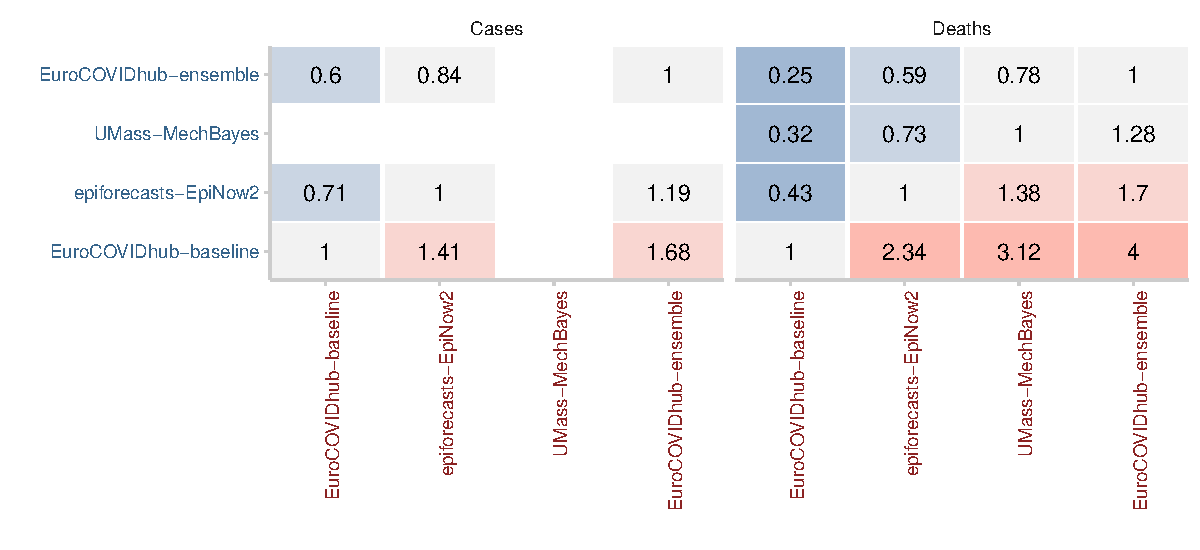
\includegraphics[width=1\linewidth]{manuscript_files/figure-latex/pairwise-plot-1} 

}

\caption[Ratios of mean scores based on overlapping forecast sets]{Ratios of mean scores based on overlapping forecast sets. When interpreting the plot one should look at the model on the y-axis, and the model on the x-axis is the one it is compared against. If a tile is blue, then the model on the y-axis performed better. If it is red, the model on the x-axis performed better in direct comparison. In the example above, the EuroCOVIDhub-ensemble performs best (it only has values smaller than one), while the EuroCOVIDhub-baseline performs worst (and only has values larger than one). For cases, the UMass-MechBayes model is excluded as there are no case forecasts available and therefore the set of overlapping forecasts is empty.}\label{fig:pairwise-plot}
\end{figure}
\end{CodeChunk}

\hypertarget{model-diagnostics}{%
\subsection{Model diagnostics}\label{model-diagnostics}}

The \pkg{scoringutils} package offers a variety of functions to aid the
user in diagnosing issues with models. For example, to detect systematic
patterns it may be useful to visualise a single metric across several
dimensions. The following produces a heatmap of bias values across
different locations and forecast targets (output shown in Figure
\ref{fig:score-heatmap}).

\begin{CodeChunk}
\begin{CodeInput}
R> score(example_continuous) |>
+   summarise_scores(by = c("model", "location", "target_type")) |>
+   plot_heatmap(x = "location", metric = "bias") + 
+     facet_wrap(~ target_type) 
\end{CodeInput}
\begin{figure}[!h]

{\centering 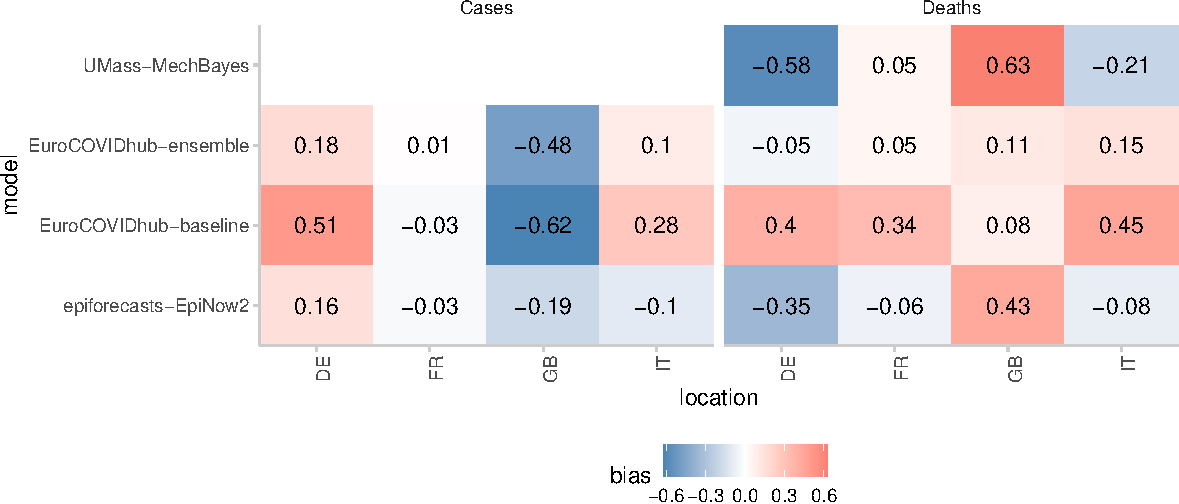
\includegraphics[width=1\linewidth]{manuscript_files/figure-latex/score-heatmap-1} 

}

\caption[Heatmap of bias values for different models across different locations and forecast targets]{Heatmap of bias values for different models across different locations and forecast targets. Bias values are bound between -1 (underprediction) and 1 (overprediction) and should be 0 ideally. Red tiles indicate an upwards bias (overprediction), while blue tiles indicate a downwards bias (under-predicction)}\label{fig:score-heatmap}
\end{figure}
\end{CodeChunk}

For quantile-based forecasts, it is helpful to visualise the
decomposition of the weighted interval score into its components:
dispersion, overprediction and underprediction. This can be achieved
using the function \code{plot\_wis()}, as shown in Figure
\ref{fig:wis-components}

\begin{CodeChunk}
\begin{CodeInput}
R> score(example_quantile) |>
+   summarise_scores(by = c("model", "target_type")) |>
+   plot_wis(relative_contributions = FALSE) + 
+   facet_wrap(~ target_type, 
+              scales = "free_x") 
\end{CodeInput}
\end{CodeChunk}

\begin{CodeChunk}
\begin{figure}[!h]

{\centering 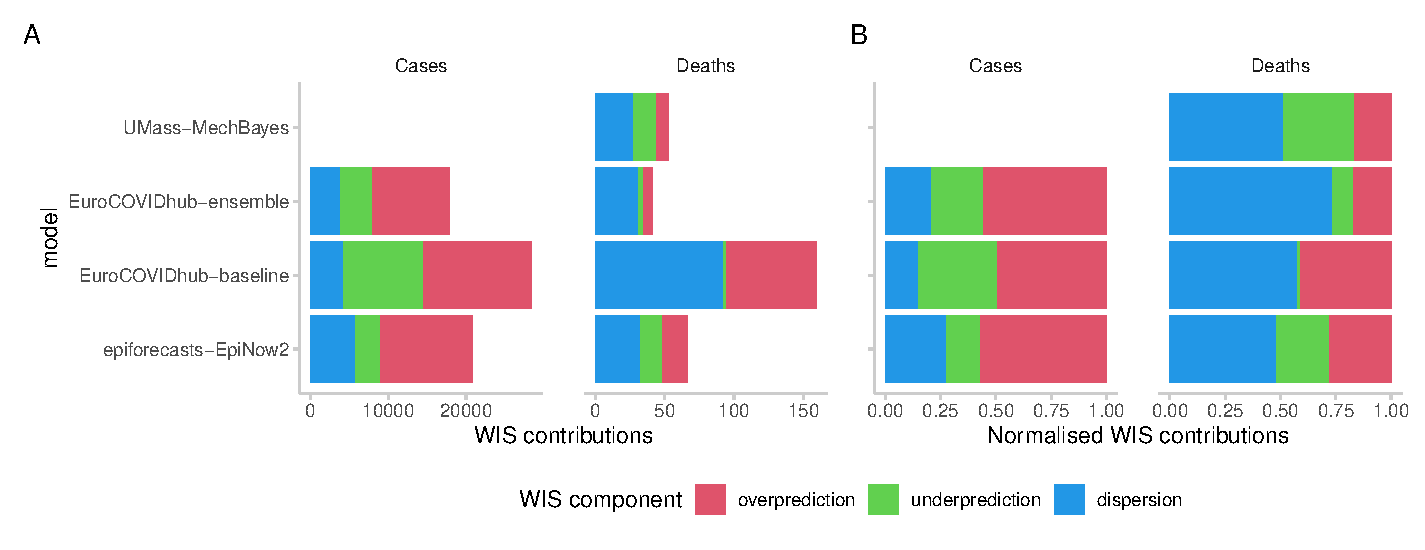
\includegraphics[width=1\linewidth]{manuscript_files/figure-latex/wis-components-1} 

}

\caption[Decomposition of the weighted interval score (WIS) into dispersion, overprediction and underprediction]{Decomposition of the weighted interval score (WIS) into dispersion, overprediction and underprediction. A: absolute contributions, B: contributions normalised to 1.}\label{fig:wis-components}
\end{figure}
\end{CodeChunk}

Special attention should be given to calibration. The most common way of
assessing calibration (more precisely: probabilistic calibration) are
PIT histograms, as explained in section \ref{probabilistic-calibration}.
Ideally, PIT values should be uniformly distributed after the
transformation.

We can compute PIT values in the following way:

\begin{CodeChunk}
\begin{CodeInput}
R> example_continuous |>
+   pit(by = "model") 
\end{CodeInput}
\begin{CodeOutput}
                     model pit_value
  1: EuroCOVIDhub-baseline     0.025
  2: EuroCOVIDhub-baseline     0.525
  3: EuroCOVIDhub-baseline     0.000
  4: EuroCOVIDhub-baseline     0.000
  5: EuroCOVIDhub-baseline     0.200
 ---                                
883:       UMass-MechBayes     0.950
884:       UMass-MechBayes     0.500
885:       UMass-MechBayes     0.100
886:       UMass-MechBayes     0.450
887:       UMass-MechBayes     0.100
\end{CodeOutput}
\end{CodeChunk}

and create PIT histograms using the function \code{plot\_pit()}. The
output of the following is shown in Figure \ref{fig:pit-plots}:

\begin{CodeChunk}
\begin{CodeInput}
R> example_continuous |>
+   pit(by = c("model", "target_type")) |>
+   plot_pit() + 
+   facet_grid(target_type ~ model)
\end{CodeInput}
\begin{figure}[!h]

{\centering 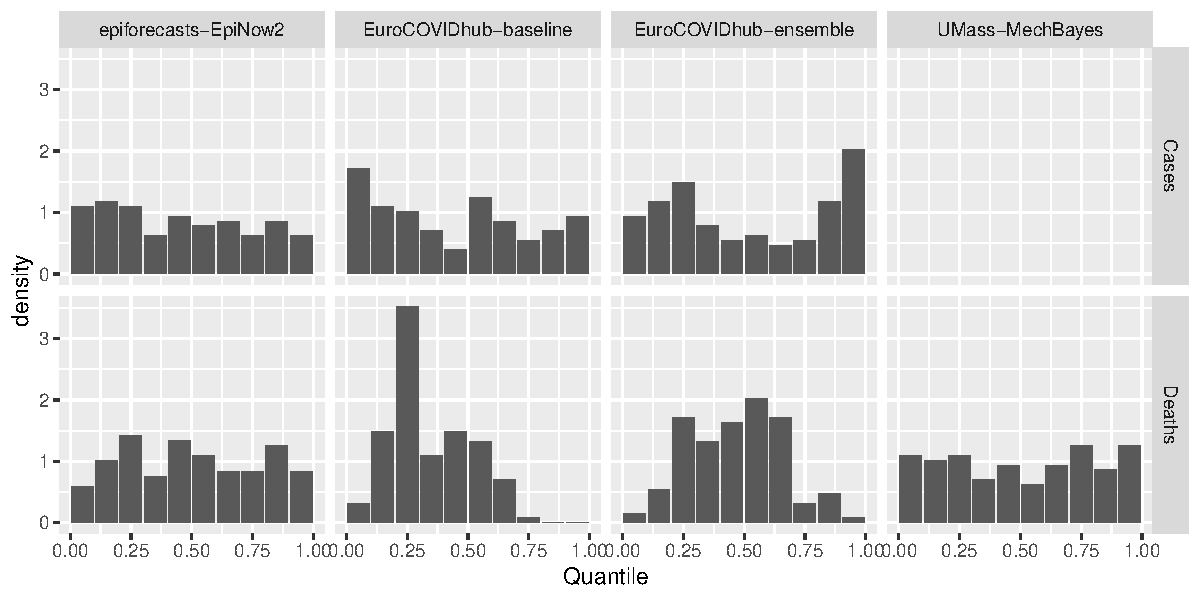
\includegraphics[width=1\linewidth]{manuscript_files/figure-latex/pit-plots-1} 

}

\caption[PIT histograms of all models stratified by forecast target]{PIT histograms of all models stratified by forecast target. Histograms should ideally be uniform. A u-shape usually indicates overconfidence (forecasts are too narrow), a hump-shaped form indicates underconfidence (forecasts are too uncertain) and a triangle-shape indicates bias.}\label{fig:pit-plots}
\end{figure}
\end{CodeChunk}

We can also look at interval and quantile coverage plots (explained in
more detail in section \ref{probabilistic-calibration}) using the
functions \code{plot\_interval\_coverage()} and
\code{plot\_quantile\_coverage()}. These plots require that the columns
``range'' and ``quantile'', respectively, be present in the scores to
plot, and therefore need to be included in the \texttt{by} argument when
summarising scores. The output of the following is shown in Figure
\ref{fig:coverage}.

\begin{CodeChunk}
\begin{CodeInput}
R> cov_scores <- score(example_quantile) |>
+   summarise_scores(by = c("model", "target_type", "range", "quantile"))
R> 
R> plot_interval_coverage(cov_scores) + 
+   facet_wrap(~ target_type)
R> 
R> plot_quantile_coverage(cov_scores) + 
+   facet_wrap(~ target_type)
\end{CodeInput}
\end{CodeChunk}

\begin{CodeChunk}
\begin{figure}[!h]

{\centering 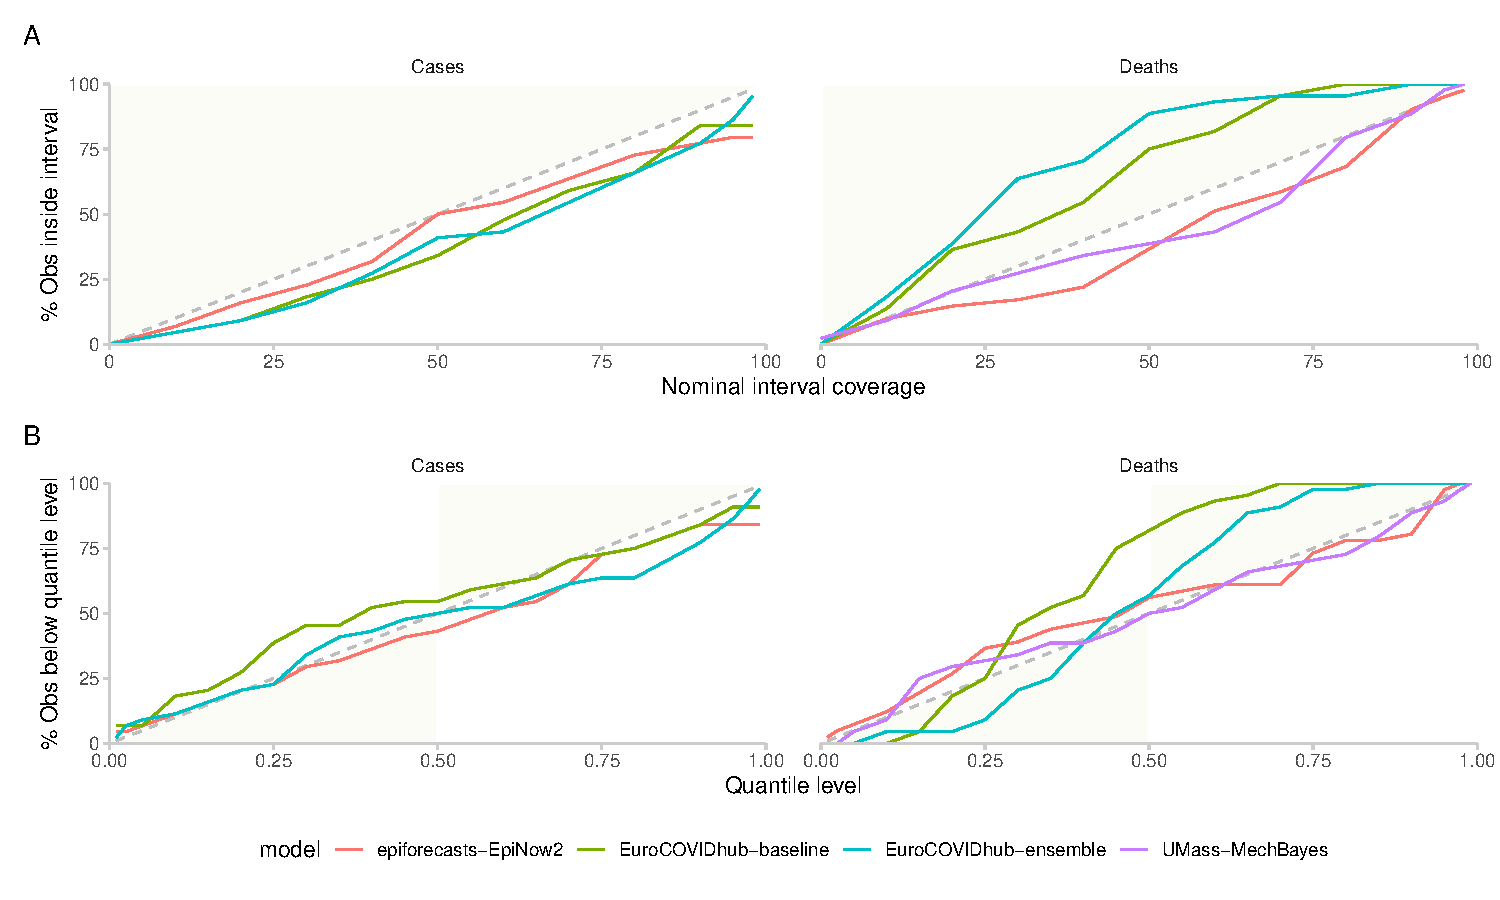
\includegraphics[width=1\linewidth]{manuscript_files/figure-latex/coverage-1} 

}

\caption[Interval coverage (A) and quantile coverage (B) plots]{Interval coverage (A) and quantile coverage (B) plots. Areas shaded in green indicate that the forecasts are too wide (i.e. underconfident), while areas in white indicate that the model is overconfident and generates too narrow predictions intervals.}\label{fig:coverage}
\end{figure}
\end{CodeChunk}

It may sometimes be interesting to see how different scores correlate
with each other. We can examine this using the function
\code{correlation()}. When dealing with quantile-based forecasts, it is
important to call \code{summarise\_scores()} before \code{correlation()}
in order to summarise over quantiles before computing correlations. The
plot resulting from the following code is shown in Figure
\ref{fig:correlation-plot}.

\begin{CodeChunk}
\begin{CodeInput}
R> correlations <- example_quantile |>
+   score() |>
+   summarise_scores() |>
+   correlation() 
R> 
R> correlations |>
+   glimpse()
\end{CodeInput}
\begin{CodeOutput}
Rows: 7
Columns: 8
$ interval_score     <dbl> 1.00, 0.46, 0.28, 0.94, -0.34, 0.11, 0.99
$ dispersion         <dbl> 0.46, 1.00, 0.15, 0.32, -0.12, 0.11, 0.54
$ underprediction    <dbl> 0.28, 0.15, 1.00, -0.03, -0.33, -0.35, 0.~
$ overprediction     <dbl> 0.94, 0.32, -0.03, 1.00, -0.25, 0.22, 0.90
$ coverage_deviation <dbl> -0.34, -0.12, -0.33, -0.25, 1.00, 0.06, -~
$ bias               <dbl> 0.11, 0.11, -0.35, 0.22, 0.06, 1.00, 0.10
$ ae_median          <dbl> 0.99, 0.54, 0.34, 0.90, -0.38, 0.10, 1.00
$ metric             <chr> "interval_score", "dispersion", "underpre~
\end{CodeOutput}
\begin{CodeInput}
R> correlations |>
+   plot_correlation()
\end{CodeInput}
\begin{figure}[!h]

{\centering 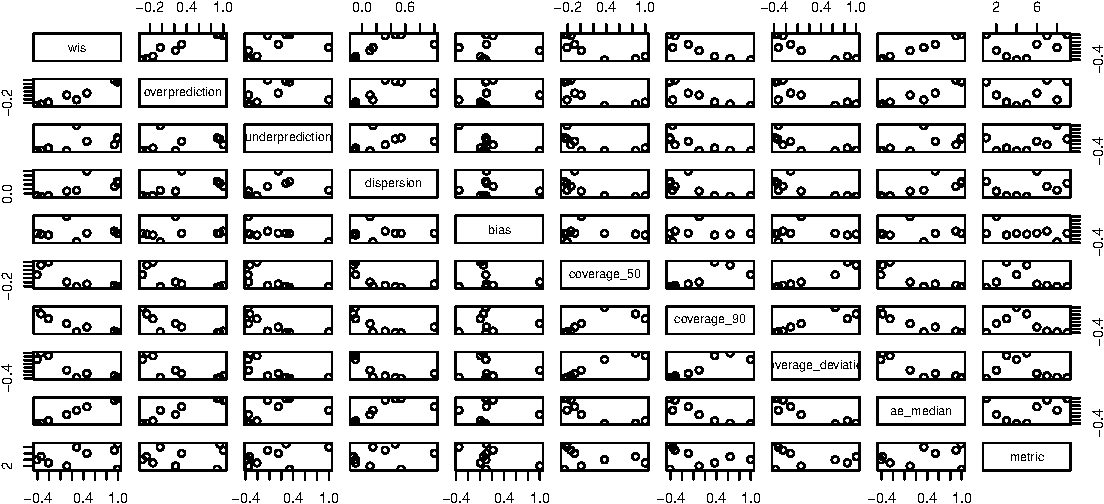
\includegraphics[width=1\linewidth]{manuscript_files/figure-latex/correlation-plot-1} 

}

\caption[Correlation between different scores]{Correlation between different scores}\label{fig:correlation-plot}
\end{figure}
\end{CodeChunk}

\hypertarget{summary-and-discussion}{%
\subsection{Summary and discussion}\label{summary-and-discussion}}

Forecast evaluation is invaluable to understanding and improving current
forecasts. The \pkg{scoringutils} package aims to facilitate this
process and make it easier, even for less experienced users. It provides
a fast, flexible and convenient evaluation framework based on
\texttt{data.frame}s, but also makes a set of scoring functions
available to more experienced users to be used in other packages or
pipelines. A set of visualisations and plotting functions help with
diagnosing issues with models and allow for thorough comparison between
different forecasting approaches.

The package is still under active development and we warmly welcome
contributions to \pkg{scoringutils}. In the future we hope to extend the
number of scoring metrics supported. This includes spherical scoring
rules
\citep{gneitingStrictlyProperScoring2007, joseCharacterizationSphericalScoring2009, macheteContrastingProbabilisticScoring2012},
evaluation of multinomial prediction tasks, as well as a broader range
of scoring metrics for point forecasts. We also plan to expand the
plotting functionality and hope to make templates available for
automated scoring reports.

\hypertarget{acknowledgments}{%
\subsection{Acknowledgments}\label{acknowledgments}}

Funding statements

NIB received funding from the Health Protection Research Unit (grant
code NIHR200908). HG MISSING. AC acknowledges funding by the NIHR, the
Sergei Brin foundation, USAID, and the Academy of Medical Sciences. EvL
acknowledges funding by the National Institute for Health Research
(NIHR) Health Protection Research Unit (HPRU) in Modelling and Health
Economics (grant number NIHR200908) and the European Union's Horizon
2020 research and innovation programme - project EpiPose (101003688).
SF's work was supported by the Wellcome Trust (grant: 210758/Z/18/Z),
and the NIHR (NIHR200908). SA's work was funded by the Wellcome Trust
(grant: 210758/Z/18/Z). This study is partially funded by the National
Institute for Health Research (NIHR) Health Protection Research Unit in
Modelling and Health Economics, a partnership between UK Health Security
Agency and Imperial College London in collaboration with LSHTM (grant
code NIHR200908); and acknowledges funding from the MRC Centre for
Global Infectious Disease Analysis (reference MR/R015600/1), jointly
funded by the UK Medical Research Council (MRC) and the UK Foreign,
Commonwealth \& Development Office (FCDO), under the MRC/FCDO Concordat
agreement and is also part of the EDCTP2 programme supported by the
European Union. Disclaimer: ``The views expressed are those of the
author(s) and not necessarily those of the NIHR, UKHSA or the Department
of Health and Social Care. We thank Community Jameel for Institute and
research funding

\newpage

\appendix

\hypertarget{appendix-detailed-information-on-metrics}{%
\section*{(APPENDIX) Detailed Information on
Metrics}\label{appendix-detailed-information-on-metrics}}
\addcontentsline{toc}{section}{(APPENDIX) Detailed Information on
Metrics}

\begin{CodeChunk}

\begin{longtable}[t]{>{\raggedright\arraybackslash}p{1.1in}>{\raggedright\arraybackslash}p{4.625in}}
\caption{\label{tab:score-table-detailed}Detailed explanation of all the metrics,}\\
\toprule
Metric & Explanation\\
\midrule
\endfirsthead
\caption[]{Detailed explanation of all the metrics, \textit{(continued)}}\\
\toprule
Metric & Explanation\\
\midrule
\endhead

\endfoot
\bottomrule
\endlastfoot
CRPS (Continuous) ranked probability score & The crps is a proper scoring rule that generalises the absolute error to probabilistic forecasts. It measures the 'distance' of the predictive distribution to the observed data-generating distribution. The CRPS is given as
  $$\text{CRPS}(F, y) = \int_{-\infty}^\infty \left( F(x) - 1(x \geq y) \right)^2 dx,$$
  where y is the true observed value and F the CDF of predictive distribution. Often An alternative representation is used:
  $$ \text{CRPS}(F, y) = \frac{1}{2} \mathbb{E}_{F} |X - X'| - \mathbb{E}_P |X - y|,$$ where $X$ and $X'$ are independent realisations from the predictive distributions $F$ with finite first moment and $y$ is the true value. In this represenation we can simply replace $X$ and $X'$ by samples sum over all possible combinations to obtain the CRPS.
  For integer-valued forecasts, the RPS is given as
  $$ \text{RPS}(F, y) = \sum_{x = 0}^\infty (F(x) - 1(x \geq y))^2. $$

\cellcolor{gray!6}{  \textbf{Usage and caveats} Smaller values are better. The crps is a good choice for most practical purposes that involve decision making, as it takes the entire predictive distribution into account. If two forecasters assign the same probability to the true event $y$, then the forecaster who assigned high probability to events far away from $y$ will still get a worse score. The crps (in contrast to the log score) can at times be quite lenient towards extreme mispredictions. Also, due to it's similarity to the absolute error, the level of scores depend a lot on the absolute value of what is predicted, which makes it hard to compare scores of forecasts for quantities that are orders of magnitude apart.}\\
\addlinespace
Log score & The Log score is a proper scoring rule that is simply compuated as the log of the predictive density evaluated at the true observed value. It is given as
  $$ \text{log score} = \log f(y), $$
  where $f$ is the predictive density function and y is the true value. For integer-valued forecasts, the log score can be computed as
  $$ \text{log score} = \log p_y, $$
  where $p_y$ is the probability assigned to outcome p by the forecast F.

  \textbf{Usage and caveats}: Larger values are better, but sometimes the sign is reversed. The log score is ensitive to outliers, as individual negative log score contributions quickly can become very large if the event falls in the tails of the predictive distribution, where $f(y)$ (or $p_y$) is close to zero. Whether or not that is desirable depends ont the application. In scoringutils, the log score cannot be used for integer-valued forecasts, as the implementation requires a predictive density. In contrast to the crps, the log score is a local scoring rule: it's value only depends only on the probability that was assigned to the actual outcome. This property may be desirable for inferential purposes, for example in a Bayesian context (Winkler et al., 1996). In settings where forecasts inform decision making, it may be more appropriate to score forecasts based on the entire predictive distribution.\\
\addlinespace
WIS (Weighted) interval score & The (weighted) interval score is a proper scoring rule for quantile forecasts that converges to the crps for an increasing number of intervals. The score can be decomposed into a sharpness (uncertainty) component and penalties for over- and underprediction. For a single interval, the score is computed as
  $$IS_\alpha(F,y) = (u-l) + \frac{2}{\alpha} \cdot (l-y) \cdot 1(y \leq l) + \frac{2}{\alpha} \cdot (y-u) \cdot 1(y \geq u), $$
  where $1()$ is the indicator function, $y$ is the true value, and $l$ and $u$ are the $\frac{\alpha}{2}$ and $1 - \frac{\alpha}{2}$ quantiles of the predictive distribution $F$, i.e. the lower and upper bound of a single prediction interval. For a set of $K$ prediction intervals and the median $m$, the score is computed as a weighted sum,
  $$WIS = \frac{1}{K + 0.5} \cdot (w_0 \cdot |y - m| + \sum_{k = 1}^{K} w_k \cdot IS_{\alpha}(F, y)),$$
  where $w_k$ is a weight for every interval. Usually, $w_k = \frac{\alpha_k}{2}$ and $w_0 = 0.5$.

  \textbf{Usage and caveats}:
\cellcolor{gray!6}{  Smaller scores are better. Applicable to all quantile forecasts, takes the entire predictive distribution into account. Just as the crps, the wis is based on measures of absolute error. When averaging across multiple targets, it will therefore be dominated by targets with higher absolute values. The decomposition into sharpness, over- and underprediction make it easy to interpret scores and use them for model improvement.}\\
\addlinespace
DSS Dawid-Sebastiani score & The Dawid-Sebastiani-Score is a proper scoring rule proposed that only relies on the first moments of the predictive distribution and is therefore easy to compute. It is given as

  $$\text{dss}(F, y) = \left( \frac{y - \mu}{\sigma} \right)^2 + 2 \cdot \log \sigma,$$
  where $F$ is the predictive distribution with mean $\mu$ and standard deviation $\sigma$ and $y$ is the true observed value.

  \textbf{Usage and caveats} The dss is applicable to continuous and integer forecasts and easy to compute. Apart from the ease of computation we see little advantage in using it over other scores.\\
\addlinespace
Brier score & Proper scoring rule for binary forecasts. The Brier score is computed as
  $$\text{Brier Score} = \frac{1}{N} \sum_{n = 1}^{N} (f_n - y_n),$$
  where $f_n$, with $n = 1, \dots, N$ are the predicted probablities that the corresponding events, $y_n \in (0, 1)$ will be equal to one.)

\cellcolor{gray!6}{  \textbf{Usage}: Applicable to all binary forecasts.}\\
\addlinespace
Interval coverage & Interval coverage measures the proportion of observed values that fall in a given prediction interval range. Interval coverage for a single prediction interval range can be calculated as $$IC_{\alpha} = \text{nominal coverage} - \text{empirical coverage},$$
  where nominal coverage is $1 - \alpha$ and empirical coverage is the proportion of true values actually covered by all $1 - \alpha$ prediction intervals.

  To summarise interval coverage over different over multiple interval ranges, we can compute coverage deviation defined as the mean interval coverage over all $K$ interval ranges $\alpha_k$ with $k = 1, \dots, K$:
  $$\text{Coverage deviation} = \frac{1}{K} \sum_{k = 1}^{K} \text{IC}_{\alpha_k}$$

  \textbf{Usage}: Interval coverage for a set of chosen intervals, (e.g. 50\% and 90\%) gives a good indication of marginal calibration and is easy to interpret. Reporting coverage deviation has the advantage of summarising calibration in a single number, but loses some of the nuance.\\
\addlinespace
Quantile coverage & Quantile coverage for a given quantile level is the proportion of true values smaller than the predictions corresponding to that quantile level.

\cellcolor{gray!6}{  \textbf{Usage}: Quantile coverage is similar to interval coverage, but conveys more information. For example, it allows us to look at the 5\% and 95\% quantile separately, instead of jointly at the 90\% prediction interval). This helps to diagnose whether it is the upper or lower end of a prediction interval that is causing problems. Plots of quantile coverage are conceptually very similar to PIT histograms.}\\
\addlinespace
Probability integral transform (PIT) & The probability integral transform (PIT, Dawid 1984) represents a succinct way to visualise deviations between the predictive distribution $F$ and the true data-generating distribution $G$. The idea is to transform the observed values such that agreement between forecasts and data can then be examined by observing whether or not the transformed values follow a uniform distribution. The PIT is given by
  $$u = F (y),$$
  where $u$ is the transformed variable and $F(y)$ is the predictive distribution $F$ evaluated at the true observed value $y$. If $F = G$, then $u$ follows a uniform distribution.

  For integer outcomes, the PIT is no longer uniform even when forecasts are ideal. Instead, a randomised PIT can be used:
  $$u = P(y) + v \cdot (P(y) - P(y - 1) ),$$
  where $y$ is again the observed value $P()$ is the cumulative probability assigned to all values smaller or equal to $y$ (where $P(-1) = 0$ by definition, and $v$ is a standard uniform variable independent of $y$. If $P$ is equal to the true data-generating distribution function, then $u$ is standard uniform.  also propose a non-randomised version of the PIT for count data that could be used alternatively.

  \textbf{Usage}:
  One can plot a histogram of $u$ values to look for deviations from uniformity. U-shaped histograms often result from predictions that are too narrow, while hump-shaped histograms indicate that predictions may be too wide. Biased predictions will usually result in a triangle-shaped histogram. One can also test for deviations from normality, using for example an Anderson-Darling test. This, however, proves to be overly strict in practice and even slight deviations from perfect calibration are punished in a way that makes it very hard to compare models at all. In addition, errors from forecasts may be correlated (i.e. forecasts made on a given date), potentially violating the assumptions of the Anderson-Darling test. We therefore do not recommend it for most use cases.\\
\addlinespace
Sharpness & Sharpness is the ability to produce narrow forecasts and is a feature of the forecasts only and does not depend on the observations. Sharpness is therefore only of interest conditional on calibration: a very precise forecast is not useful if it is clearly wrong.

  As suggested by Funk et al. (2019), we measure sharpness for continuous and integer forecasts represented by predictive samples as the normalised median absolute deviation about the median (MADN) ), i.e.
  $$ S(F) = \frac{1}{0.675} \cdot \text{median}(|x - \text{median(x)}|), $$
  where $x$ is the vector of all predictive samples and $\frac{1}{0.675}$ is a normalising constant. If the predictive distribution $F$ is the CDF of a normal distribution, then sharpness will equal the standard deviation of $F$.

\cellcolor{gray!6}{  For quantile forecasts we can directly use the sharpness component of the weighted interval score. Sharpness is then simply the weighted mean of the widths of the central prediction intervals.}\\
\addlinespace
Bias & Bias is a measure of the tendency of a forecaster to over- or underpredict. For continuous forecasts, bias is given as
  $$B(F, y) = 1 - 2 \cdot (F (y)), $$
  where $F$ is the CDF of the predictive distribution and $y$ is the observed value.

  For integer-valued forecasts, bias can be calculated as
  $$B(P, y) = 1 - (P(y) + P(y + 1)), $$
  where $P(y)$ is the cumulative probability assigned to all outcomes smaller or equal to $y$.

  For quantile forecasts, Bias can be calculated as the maximum percentile rank for which the prediction is smaller than $y$, if the true value is smaller than the median of the predictive distribution. If the true value is above the median of the predictive distribution, then bias is the minimum percentile rank for which the corresponding quantile is still larger than the true value. If the true value is exactly the median, bias is zero. For a large enough number of quantiles, the percentile rank will equal the proportion of predictive samples below the observed true value, and this metric coincides with the one for continuous forecasts.

  \textbf{Usage}:
  In contrast to the over- and underprediction penalties of the interval score it is bound between 0 and 1 and represents the tendency of forecasts to be biased rather than the absolute amount of over- and underprediction. It is therefore a more robust measurement, but harder to interpet. It largely depends on the application whether one is more interested in the tendency to be biased or in the absolute value of over- and underpredictions.\\
\addlinespace
Mean score ratio & The mean score ratio is used to compare two models on the overlapping set of forecast targets for which both models have made a prediction. The mean score ratio is calculated as the mean score achieved by the first model over the mean score achieved by the second model. More precisely, for two models $i, j$, we determine the set of overlapping forecasts, denoted by $\mathcal{A}_{ij}$ and compute the mean score ratio $\theta_{ij}$ as
  $$\theta_{ij} =\frac{\text{mean score model } i \text{ on } \mathcal{A}_{ij}}{\text{mean score model } j \text{ on } \mathcal{A}_{ij}}.$$
  The mean score ratio can in principle be computed for any arbitrary score.

  \textbf{Usage}:
\cellcolor{gray!6}{  Mean scores ratios are usually calculated in the context of pairwise comparisons, where a set of models is compared by looking at mean score ratios of all possible parings. Whether smaller or larger values are better depends on the orientation of the original score used}\\
\addlinespace
Relative skill & Relative skill scores can be used to obtain a ranking of models based on pairwise comparisons between all models. To compute the relative skill $\theta_i$ of model $i$, we take the geometric mean of all mean score ratios that involve model $i$, i.e.
  $$ \theta_{i} = \left(\prod_{m = 1}^M \theta_{im}\right)^{1/M}, $$
  where M is the number of models.

  \textbf{Usage and caveats}:
  Relative skill is a helpful way to obtain a model ranking. Whether smaller or larger values are better depends on the orientation of the original score used.
  It is in principle relatively robust against biases that arise when models only forecast some of the available targets and is a reasonable way to handle missing forecasts. One possible precautionary measure to reduces issues with missing forecasts is to only compare models that have forecasted at least half of all possible targets (this ensures that there is always an overlap between models). If there is no overlap between models, the relative skill implicitly estimates how a model would have forecasted on those missing targets.\\*
\end{longtable}

\end{CodeChunk}

\newpage

\bibliography{references.bib,scoringutils-paper.bib}



\end{document}
